\PassOptionsToPackage{dvipsnames}{xcolor}

% draft会跳过文档中的所有图片。正式导出时需要删掉draft参数。
\documentclass[12pt, a4paper, oneside]{ctexart}

\usepackage{amsmath}
\usepackage{amssymb}
\usepackage{bm}
\usepackage{graphicx}
\usepackage{mathrsfs}
\usepackage{geometry}
\usepackage{framed}
\usepackage{caption}
\usepackage{listings}
\usepackage{fancyhdr}
\usepackage{booktabs}
\usepackage{makecell}
\usepackage{indentfirst}
\usepackage{authblk}
\usepackage{multicol}
% \usepackage{draftwatermark}       % 需要应用水印时取消注释
\usepackage{enumitem}
\usepackage[hidelinks]{hyperref}
\usepackage{tikz}
\usepackage{ulem}
\usetikzlibrary{positioning, shapes.geometric}

% 分栏线宽
\columnseprule=0.4pt

% 定制第二级无序列表的点样式
\setlist[itemize,2]{label=$\diamond$}

% 页边距
\geometry{a4paper, scale=0.8}

\pagestyle{fancy}

% 调整页眉高度,用于去除警告
\setlength{\headheight}{25pt}

\fancyhf{}      % 清空页眉页脚设置
\fancyhead[L] {
    % 工大计算机系logo
    
\includegraphics[height=7mm]{../../share/images/logo1.jpg}
}
\fancyhead[C]{《操作系统》复习}
\fancyhead[R]{\leftmark}    % 右侧页眉:当前章标题

% 页脚居中放置页码
\fancyfoot[C]{\thepage}

% 设置章节标题自动编号的格式
\ctexset{
  section/number=\chinese{section},
%   subsection/name={,},
%   subsection/number=\chinese{subsection}
}

% 行距。ctexart默认值为1.3
\linespread{1.2}

\lstset{
  language=c,
  basicstyle=\ttfamily,
  frame=single,
  % keywordstyle=\bfseries\color{NavyBlue}  % 彩色看起来怪怪的,所以注释掉了
  numbers=left, % 显示行号在左边
  numbersep=2em, % 设置行号的具体位置
  numberstyle=\footnotesize, % 缩小行号
  frame=single, % 边框
  framesep=1em % 设置代码与边框的距离
}

% \SetWatermarkText{Eslzzyl整理}            % 设置水印内容
% \SetWatermarkLightness{0.9}             % 设置水印透明度 0-1
% \SetWatermarkScale{0.8}                   % 设置水印大小 0-1

\renewcommand{\headrulewidth}{1pt}  %页眉线宽,设为0可以去页眉线
\renewcommand{\footrulewidth}{1pt}  %脚注线的宽度

\definecolor{shadecolor}{RGB}{241, 241, 255}

\title{
    
\includegraphics[width=0.3\textwidth]{../../share/images/hfut-badge.pdf}
    
    \vspace{20pt}
    《操作系统》总复习
}
\author{Eslzzyl}
\date{\today}

\newcounter{problemname}
\newenvironment{problem}{\begin{shaded}\stepcounter{problemname}\par\noindent\textbf{例题\arabic{problemname}. }}{\end{shaded}\par}
\newenvironment{solution}{\begin{shaded}\par\noindent\textbf{解答:}}{\end{shaded}\par}
% \newenvironment{solution}{\par\noindent\textbf{答案. }}{\par}
% \newenvironment{note}{\par\noindent\textbf{例题\arabic{problemname}的注记. }}{\\\par}
\newenvironment{note}{\par\noindent\textbf{注记. }}{\par}

\begin{document}

\maketitle
\newpage
\tableofcontents
\vspace{20pt}
% 如果在目录处有备注,可以写在这里。

\newpage

\section{计算机系统概述}

本章主要是选择题。

\subsection{操作系统的基本概念}

\subsubsection{操作系统的概念}

计算机系统\textbf{自上而下}可分为4层:
\begin{enumerate}
  \item 用户
  \item 应用程序
  \item 操作系统
  \item 硬件
\end{enumerate}

操作系统的\textbf{定义}:操作系统是一组管理和控制计算机软件和硬件资源,合理组织计算机系统工作流程,以及方便用户使用的\textbf{程序的集合}。

OS是计算机系统中最基本的系统软件。

\subsubsection{操作系统的特征}

四大基本特征:
\begin{itemize}
  \item {\bf 并发(Concurrence)}
  \begin{itemize}
    \item 并发:多个事件在同一时间间隔内发生。
    \item 并行:多个事件在同一时刻发生。
  \end{itemize}
  操作系统的并发性是通过分时得以实现的。
  \item {\bf 共享(Sharing)}
  \begin{itemize}
    \item 互斥共享方式
    \item 同时访问方式
  \end{itemize}
  \item {\bf 虚拟(Virtual)}
  
  虚拟技术有两种实现方式:
  \begin{itemize}
    \item 时分复用技术,如处理器的分时共享;
    \item 空分复用技术,如虚拟存储器。
  \end{itemize}
  \item {\bf 异步(Asynchronism)}
  
  多道程序环境下,程序的执行是走走停停的,即以不可知的速度向前推进,这就是进程的异步性。OS必须保证在相同的运行环境下,进程多次运行的结果是一致的。
\end{itemize}

并发和共享是OS的\textbf{最基本特性}。二者是相互依存的。

\subsubsection{操作系统的目标和功能}

\begin{enumerate}
  \item 系统资源的\textbf{管理}者
  \begin{itemize}
    \item 处理机管理,也就是对进程的管理,包括
    \begin{itemize}
      \item 进程控制
      \item 进程同步
      \item 进程通信
      \item 死锁处理
      \item 处理机调度
    \end{itemize}
    \item 存储器管理
    \begin{itemize}
      \item 内存分配与回收
      \item 地址映射
      \item 内存保护和共享
      \item 内存扩充
    \end{itemize}
    \item 文件管理
    \begin{itemize}
      \item 文件存储空间的管理
      \item 目录管理
      \item 文件读写管理和保护
    \end{itemize}
    \item 设备管理
    \begin{itemize}
      \item 缓冲管理
      \item 设备分配
      \item 设备处理
      \item 虚拟设备
    \end{itemize}
  \end{itemize}
  \item 作为用户和硬件系统之间的\textbf{接口}
  \begin{itemize}
    \item 命令接口
    \begin{itemize}
      \item 联机方式:字符交互式
      \item 脱机方式:批处理式
    \end{itemize}
    \item 程序接口:由一组\textbf{系统调用}组成
  \end{itemize}

  目前最流行的GUI(图形接口)是建立在程序接口基础上的。

  \item 实现对计算机资源的\textbf{扩充}
\end{enumerate}

\subsection{操作系统发展历程}

推动OS发展的主要动力:
\begin{itemize}
  \item 不断提高计算机资源利用率
  \item 方便用户
  \item 器件的不断更新换代
  \item 计算机体系结构的发展
  \item 不断提出新的应用需求
\end{itemize}

\subsubsection{无操作系统时代(手工操作阶段)}

对计算机的所有操作采用人工操作方式完成。人工操作方式的缺点:
\begin{itemize}
  \item 用户独占全机
  \item CPU等待人工操作
\end{itemize}

由于以上两点,昂贵的机器资源在大部分时间内处于空闲状态,非常浪费。

优点:交互性好,即用户可以得到机器的立即响应。

\subsubsection{批处理系统阶段}

\textbf{批处理系统}:在计算机上加载一个专门监控软件,在其控制下,计算机
能够自动地、成批地处理一个或多个用户的一批作业。

批处理系统的特点:
\begin{itemize}
  \item 系统吞吐量大
  \item 资源利用率高
  \item 平均周转时间短
  \item 无交互能力(缺点)
\end{itemize}

\begin{enumerate}
  \item {\bf 单道批处理系统}
  
  先把一批作业输入到磁带上,在监控程序的控制下使这批作业一个接一个地处理。内存中始终只保持一道作业。

  代表系统:IBM的FMS(Fortran Monitoring System),1960s

  一定程度上改善了资源浪费,但失去了交互性。单个程序独占系统,程序I/O时CPU空等。

  单道批处理系统的特点:自动性、顺序性、单道性

  \item {\bf 多道批处理系统}
  
  出现的动力是希望提高资源利用率和系统吞吐量。

  代表系统(也是第一个):IBM的OS/360,1960s

  由作业调度程序按照一定的算法,从后备队列中选择若干个作业调入内存,使它们共享CPU资源。

  相比单道批处理系统,多道批处理系统的资源利用率更高,但仍然没有交互性。

  特点:多道性、无序性、调度性、宏观上并行、微观上串行
\end{enumerate}

\subsubsection{分时系统}

出现的动力是改善交互性。

分时系统:在一台主机上连接若干个终端,允许多个用户通过终端以交互方式共享主机资源。

代表系统:CTSS(1962)、Multics(1964)

特点:
\begin{itemize}
  \item 多路性:也叫同时性。众多联机用户可以同时使用同一台计算机
  \item 独立性:各终端用户感觉到自己独占了计算机
  \item 及时性:用户的请求能在很短时间内得到响应
  \item 交互性:用户与计算机之间可进行“会话”
\end{itemize}

\subsubsection{实时系统}

实时计算:系统的正确性不仅由计算的逻辑结果来确定,而且还取决于产生结果的时间。

常见的实时系统:
\begin{itemize}
  \item 工业控制系统、武器控制系统
  \item 信息查询系统
  \item 多媒体系统
  \item 嵌入式系统
\end{itemize}

代表系统:WinCE,嵌入式Linux,ucOSII,VxWorks等

特点:实时性、高安全性、高可靠性(效率放第二位)、整体性强、会话能力要求不高

\subsubsection{网络操作系统和分布式计算机系统}

网络操作系统:将网络中的多台计算机连接起来。

分布式计算机系统:用于管理分布式计算机系统的操作系统。

\subsubsection{个人计算机操作系统}

\subsection{操作系统运行环境}

\subsubsection{处理器运行模式}

\begin{itemize}
  \item {\bf 特权指令},指不允许用户直接使用的指令。
  \item {\bf 非特权指令},指允许用户直接使用的指令。
\end{itemize}

CPU的运行模式:
\begin{itemize}
  \item {\bf 用户态}(目态)
  \item {\bf 内核态}(核心态、管态)
\end{itemize}

CPU在内核态可以执行特权指令,在用户态则只能执行非特权指令。应用程序运行在用户态,操作系统内核运行在内核态。

大多数操作系统内核包括:
\begin{itemize}
  \item 时钟管理
  \item 中断机制
  \item 原语
  \item 系统控制的数据结构及处理
\end{itemize}

\subsubsection{中断和异常的概念}

可直接参考《组成原理》相关内容。

\subsubsection{系统调用}

在用户程序中,凡与资源有关的操作,都必须使用系统调用。系统调用由OS内核完成,运行在核心态。

程序的运行由用户态转到核心态,需要用到访管指令,是用户态指令。

\subsection{操作系统结构}

\subsubsection{分层式结构OS}

原则:将功能模块分层,层内模块可以互相调用,层间模块只允许高层调用它下面紧邻着的那层,不允许反过来。

将最靠近硬件的低层OS部分称为操作系统内核,内核通常常驻主存。

优点:
\begin{itemize}
    \item 容易保证系统的正确性,容易调试和验证。
    \item 容易扩充、维护和移植。
\end{itemize}

缺点:
\begin{itemize}
  \item 效率低下。
  \item 合理定义各层比较困难。
\end{itemize}

\subsubsection{模块化结构OS}

优点:
\begin{itemize}
    \item 提高OS设计的正确性、可理解性和可维护性
    \item 增强OS的可移植性, 加速OS的开发过程
\end{itemize}

缺点:
\begin{itemize}
    \item 结构划分和接口设计困难
    \item 模块之间调用关系复杂,牵一发而动全身
    \item 各个模块的设计齐头并进,很难确定发展顺序
\end{itemize}

\subsubsection{微内核OS}

将OS划分为两大部分:
\begin{itemize}
    \item 微内核,只提供客户-服务器通信机制和与硬件紧密相关的较基本的功能
    \item 提供各类服务的一组服务器进程
\end{itemize}

OS采用C/S模式提供各类操作系统服务。微内核运行在内核态,其他服务器进程运行在用户态,这样服务器进程崩溃不会影响到微内核。

优点:
\begin{itemize}
    \item 灵活、容易移植、容易扩展、可靠
    \item 支持分布式系统和网络系统
\end{itemize}

缺点:还是效率低下(远不及宏内核快)。

现代主流操作系统已经不是纯粹的宏内核了,而是混合结构。

\subsection{操作系统引导}

过程如下:
\begin{enumerate}
  \item 激活CPU,CS:IP自动指向FFFF0H。这个地址接近内存顶部,只剩下16字节,放不下程序,于是用一条JMP指令跳转到BIOS。跳转后,读取ROM中的boot程序,将IR设为BIOS的第一条指令,开始执行BIOS。
  \item 硬件自检。这一步称为POST(Power-on Self Test)。有故障发出蜂鸣并中止启动,无故障则继续。
  \item BIOS读取引导顺序表,CPU将表上第一位的存储设备的引导扇区加载到内存。
  \item 加载MBR。CPU顺序检查引导表,如果当前设备不可引导,就检查下一个设备。MBR的作用是指出硬盘的哪个主分区含有操作系统。
  \item 扫描硬盘的分区表,加载活动分区。
  \item 加载分区引导记录PBR。PBR是指活动分区的第一个扇区。PBR指出了该分区下操作系统引导程序的位置。
  \item 根据PBR加载OS启动程序。
  \item 加载OS。
\end{enumerate}

引导程序的可分两类:
\begin{itemize}
  \item 一种是位于ROM中的自举程序(是BIOS的一部分),用于启动具体的设备;
  \item 另一种是位于装有OS的磁盘的活动分区的引导扇区中的引导程序(称为启动管理器,Boot Manager),用于引导操作系统。
\end{itemize}

\subsection{虚拟机}

有两种虚拟化方法:
\begin{itemize}
  \item 第一类虚拟机管理程序,直接运行在硬件上,其上运行操作系统。每个操作系统都认为自己运行在裸机硬件上。这种技术也叫裸金属架构。
  \item 第二类虚拟机管理程序,其实是运行在宿主操作系统上的一个程序,但仍然伪装成一台完整的计算机。x86平台上的第一个二类虚拟机管理程序是VMware Workstation。这种技术也叫寄居架构。
\end{itemize}

\section{进程与线程}

\textcolor{red}{重点。信号量进程同步、进程调度算法、死锁容易出综合题。}

\subsection{进程与线程}

\subsubsection{进程的概念和特征}

(传统OS中)进程的\textbf{定义}:进程是进程实体的运行过程,是系统进行资源分配和调度的一个独立单位。

进程实体=程序段+相关的数据段+PCB。PCB是进程存在的\textbf{唯一标志}。

进程的特征(一般不考,理解即可):
\begin{itemize}
    \item {\bf 动态性}:进程有生命周期,而程序只是一组有序指令的集合,是静态的。这是进程的\textbf{最基本}的特征。
    \item {\bf 并发性}:指多个进程可以同时存在于内存中,且能在一段时间内同时运行。
    \item {\bf 独立性}:进程实体是一个能独立运行、独立获得资源和独立接受调度的基本单位。
    \item {\bf 异步性}:进程按照各自独立的、不可预知的速度向前推进。
\end{itemize}

\subsubsection{进程的状态与转换}

前3种是基本状态。
\begin{enumerate}
  \item {\bf 运行态}。进程正在运行。单处理器系统中,同一时刻只有一个进程处于运行态。
  \item {\bf 就绪态}。进程已经获得了除处理机外的所有资源,一旦得到处理机,就立即运行。所有就绪进程排成一个就绪队列。
  \item {\bf 阻塞态}。也叫等待态。进程因资源不可用或等待I/O而暂停运行的状态。即使处理机空闲,也无法运行。可以根据阻塞原因设置多个阻塞队列。
  \item {\bf 创建态}。进程正在创建,尚未就绪。
  \item {\bf 终止态}。进程正常结束或因其他原因退出,正在消失。OS此时进行一些资源回收工作,完成后就彻底结束进程。
\end{enumerate}

这5种状态的转换关系见图\ref{process_state_transition}。

\begin{figure}
  \centering
  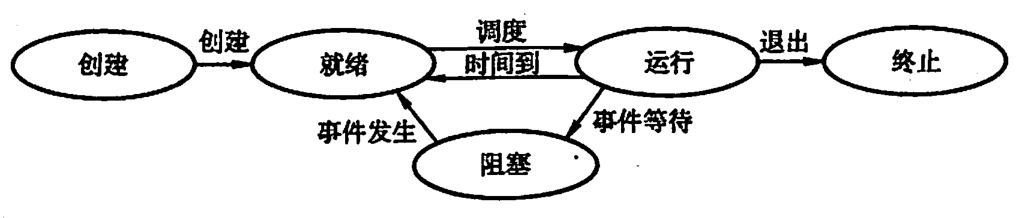
\includegraphics[width=0.7\textwidth]{./images/process_state_transition.png}
  \caption{5种进程状态的转换}
  \label{process_state_transition}
\end{figure}

注意:进程从运行态转换到阻塞态是主动的行为,从阻塞态转换到就绪态是被动的行为。

\subsubsection{进程的组成}

进程实体=程序段+相关的数据段+PCB。本节主要介绍PCB。

PCB包括如下4部分内容:
\begin{itemize}
  \item 进程描述信息。
  \item 进程控制和管理信息。
  \item 资源分配清单。
  \item 处理机相关信息。
\end{itemize}

\subsubsection{进程控制}

本节主要介绍进程的创建、中止、阻塞和唤醒原语的过程。似乎不太重要,暂略。

\subsubsection{进程的通信}

\begin{itemize}
  \item 共享存储
  \begin{itemize}
    \item 分类
    \begin{itemize}
        \item 基于共享数据结构的通信方式
        \item 基于共享存储区的通信方式
    \end{itemize}
    \item 特点
    \begin{itemize}
        \item 适合大量的数据快速交换
        \item 程序员负担重
    \end{itemize}
  \end{itemize}
  \item 消息传递
  \begin{itemize}
    \item 分类:
    \begin{itemize}
        \item 直接通信方式
        \item 间接通信方式:通过信箱(mailbox)通信
        \begin{itemize}
            \item 公有信箱
            \item 私有信箱
            \item 共享信箱
        \end{itemize}
    \end{itemize}
    \item 特点:
    \begin{itemize}
        \item 操作系统隐藏通信细节
        \item 通信程序简单
        \item 可以跨网络传输
        \item 灵活
    \end{itemize}
  \end{itemize}
  \item 管道:通过一个固定大小的共享文件实现通信。UNIX首创。
\end{itemize}

\subsubsection{线程和多线程模型}

\begin{enumerate}
  \item {\bf 传统进程的两个基本属性}
  
  \begin{itemize}
    \item 是拥有资源的独立单位
    \item 是调度和分派的基本单位
  \end{itemize}

  \item {\bf 线程的特点}
  
  \begin{itemize}
    \item 是能独立运行的基本单位,且切换代价远小于进程。
    \item 线程不拥有系统资源,而是仅拥有一点必不可少的、能保证独立运行的资源。
    \item 多个线程可以共享一个进程的资源
  \end{itemize}

  \item {\bf 线程的实现}
  
  \begin{itemize}
    \item {\bf 用户级线程 ULT}:无须内核支持,与内核无关,甚至内核不知道此类线程的存在。调度以进程为单位进行。
    \item {\bf 内核级线程 KLT}:在内核的支持下运行。调度以线程为单位进行。
  \end{itemize}

  \item {\bf 多线程模型}

  \begin{itemize}
    \item {\bf 多对一模型},多个用户级线程映射到一个内核级线程。线程管理在用户空间进行,效率高。但只要有线程访问内核发生阻塞后,整个进程都会阻塞。任何时刻只有一个线程能访问内核。
    \item {\bf 一对一模型},每个用户级线程都映射到一个内核级线程。并发性能好,但每创建一个用户线程,就要对应创建一个内核线程,开销大。
    \item {\bf 多对多模型},将$n$个用户线程映射到$m$个内核级线程上,要求$n\geq m$。克服了上面两种模型的缺点,汇集了上面两种模型的优点。
  \end{itemize}
\end{enumerate}

\subsection{处理机调度}

\subsubsection{调度的概念}

调度的层次:
\begin{itemize}
  \item 高级调度:又称长程调度、作业调度、接纳调度。
  \begin{itemize}
    \item 调度对象是作业。
    \item 根据某种算法,决定将外存上处于后备队列中的哪几个作业调入内存。
    \item 仅设置在多道批处理系统中。分时系统和实时系统不设置。
    \item 调度频率低,典型时间:几分钟。
    \item 因为调度频率低,调度算法可以设计得很复杂。
  \end{itemize}
  \item 低级调度:又称进程调度或短程调度。
  \begin{itemize}
    \item 调度对象是就绪的进程或内核级线程。
    \item 根据某种算法,决定就绪队列中的哪个进程获得处理机。
    \item 这是最基本的调度方式,在各类OS中都必须设置。
    \item 调度频率高,典型时间:几十毫秒。
    \item 因为调度时间短,调度算法必须足够简单。
  \end{itemize}
  \item 中级调度:又称内存调度。
  \begin{itemize}
    \item 调度对象是就绪进程和阻塞进程。
    \item 其实就是内存对换功能。引入的主要目的是提高内存利用率和系统吞吐量。
  \end{itemize}
\end{itemize}

\subsubsection{调度的性能指标}

\begin{itemize}
  \item CPU利用率:
  \begin{equation*}
    \text{CPU利用率}=\frac{\text{CPU有效工作时间}}{\text{CPU有效工作时间+CPU空闲时间}}
  \end{equation*}
  \item 系统吞吐量:单位时间内完成作业的数量。长作业会降低吞吐量,短作业会提高吞吐量。
  \item 周转时间:从作业被提交给系统开始,到作业完成为止的时间。=等待时间+执行时间。
  \begin{itemize}
    \item 设$T_i$是第$i$个作业的周转时间,$n$为作业总数,则系统的平均周转时间定义为
    \begin{equation*}
        T=\frac{1}{n}\left[\sum_{i=1}^{n}T_i\right]
    \end{equation*}  
    \item 再设$T_{si}$是第$i$个作业的要求服务时间,则系统的平均带权周转时间定义为
    \begin{equation*}
        W=\frac{1}{n}\left[\sum_{i=1}^{n}\frac{T_i}{T_{si}}\right]
    \end{equation*}
  \end{itemize}
  \item 等待时间:进程等待处理机的时间。影响用户满意度。
  \item 响应时间:用户提交请求到系统首次产生相应的时间。
\end{itemize}

\subsubsection{调度的实现}

调度程序的组成:
\begin{itemize}
  \item 排队器
  \item 分派器
  \item 上下文切换器
\end{itemize}

\textbf{不能}进行调度的情况:
\begin{itemize}
  \item 处理中断时。
  \item 进程在OS内核临界区内。
  \item 需要完全屏蔽中断的原子操作。
\end{itemize}

\begin{problem}
  【2012统考】【24王道书本节T24,做题本P164】若某单处理器多进程系统中有多个就绪态进程,则下列关于处理机调度的叙述中,错误的是(\ \ )

  \begin{enumerate}
    \item [A. ] 在进程结束时能进行处理机调度
    \item [B. ] 创建新进程后能进行处理机调度
    \item [C. ] 在进程处于临界区时不能进行处理机调度
    \item [D. ] 在系统调用完成并返回用户态时能进行处理机调度
  \end{enumerate}
\end{problem}

\begin{solution}
  C. 王道书的解释是,对于C,只要不破坏临界资源的使用规则,就不影响。假设某进程正在独占打印机,就不能一直等其独占结束。

  王道书称A、B、D是显然的。
\end{solution}

进程调度方式
\begin{itemize}
  \item 非抢占式调度方式:适用于大多数批处理系统,不适用于分时系统和实时系统。
  \item 抢占式调度方式
\end{itemize}

\subsubsection{典型的调度算法}

\begin{enumerate}
  \item {\bf 先来先服务(FCFS)调度算法}:最简单的调度算法。既可用于作业调度,也可用于进程调度。

  特点:
  \begin{itemize}
      \item 实现简单
      \item 对长作业有利,对短作业不利
      \item 对CPU繁忙型作业有利,对I/O繁忙型作业不利
  \end{itemize}

  \item {\bf 短作业/短进程优先(SJF/SPF)调度算法}:以作业要求的服务时间长短计算优先级。作业越短,优先级越高。两个作业时间一样长时,按FCFS调度。
  
  可以抢占,也可以非抢占。

  特点:
  \begin{itemize}
      \item 实现困难,因为难以估计作业的执行时间。
      \item 有利于短作业,对长作业不利,容易使长作业饥饿。
      \item 完全没有考虑作业的紧迫程度。
      \item \textbf{这种算法的平均等待时间、平均周转时间最少}。进程的执行时间是固定的,所以周转时间取决于等待时间。该算法能使等待时间最短。
  \end{itemize}

  \item {\bf 优先级调度算法(PSA)}:由外部赋予作业相应的优先级,根据该优先级调度。高优先级作业优先运行。
  
  在这种算法中,I/O繁忙型的作业要优于计算繁忙型的作业。

  可以抢占,也可以非抢占。

  \begin{itemize}
    \item {\bf 静态优先级}:创建进程时确定,此后一直不变。
    \item {\bf 动态优先级}:运行时根据情况调整优先级。有如下大致原则:
    \begin{itemize}
      \item 系统进程>用户进程
      \item 交互型进程>非交互型进程
      \item I/O密集型进程>计算密集型进程。
      \item 进程等待时间长时,应适当提高优先级。
      \item 进程运行时间长时,应适当降低优先级。
    \end{itemize}
  \end{itemize}
  
  \item {\bf 高响应比优先调度算法(HRRN)}:基本思想是动态优先级,作业等待时间越长,优先级越高。
  
  \begin{equation*}
    \text{响应比}R_p=\frac{\text{等待时间+要求服务时间}}{\text{要求服务时间}}=\frac{\text{响应时间}}{\text{要求服务时间}}
  \end{equation*}
  以响应比作为优先级。特点:
  \begin{itemize}
      \item 既照顾了短作业,又考虑了作业到达的先后次序,不会使长作业长期得不到服务。
      \item 每次调度之前要计算响应比,系统开销加大。
  \end{itemize}

  \item {\bf 时间片轮转调度算法(RR)}:让就绪队列上的每个进程每次运行一个时间片长度。\textbf{一定是抢占式的}。

  时间片一般取略大于一次典型的交互所需要的时间,以保证及时响应。
  \begin{itemize}
      \item 时间片太长,则退化为FCFS算法
      \item 时间片太短,调度频繁,浪费资源
  \end{itemize}

  RR的主要目的是:使多个交互的用户能够及时获得响应。

  \item {\bf 优先级调度算法}:和作业调度的PSA一致。可以抢占,也可以非抢占。

  \item {\bf 多级反馈队列(MFQ)调度算法}。有如下规则:
  \begin{itemize}
    \item 设置多个就绪队列,为每个队列赋予不同的优先级,第一个队列最高,第二个次之,以此类推。
    \item 优先级越高的队列,执行时间片越小。
    \item 每个队列都采用FCFS算法。一个新进程到来时,将其放到第一个队列的末尾。轮到它执行时,如果不能在一个时间片内完成,则放入第二队列末尾,以此类推。直到放入第n个队列,按照RR算法运行。
    \item 仅当第1队列空闲时,调度程序才调度第2队列中的进程运行;仅当第$1\text{~}(i-1)$队列均空时,才会调度第i队列中的进程运行。
    \item 若第i队列的进程正在执行,此时有新进程进入优先级更高的队列,则立即暂停当前进程并将其放入第i队列的末尾,转而执行新进程。
  \end{itemize}
\end{enumerate}

常见进程调度算法的对比:见表\ref{process_handling_algorithms}

\begin{table}
  \centering
  \caption{常见进程调度算法的对比}
  \label{process_handling_algorithms}
  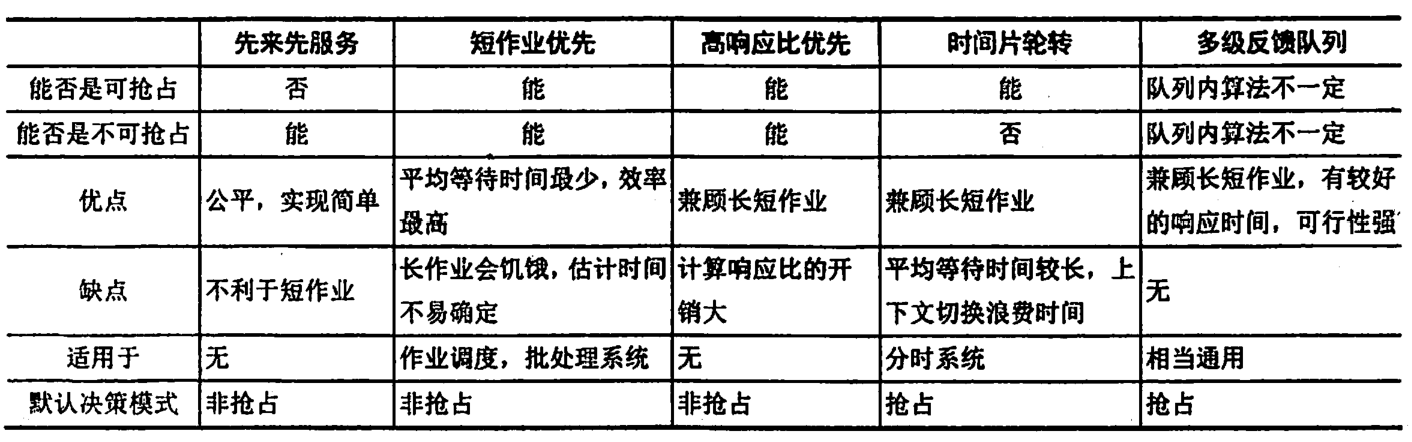
\includegraphics[width=0.9\textwidth]{./images/process_handling_algorithms.png}
\end{table}

\begin{problem}
  5个进程A,B,C,D,E分别于0,1,2,3,4时刻到达系统,要求服务时间分别为4,3,5,2,4, 请计算:
  \begin{enumerate}
    \item [(1). ] 采用FCFS时进程执行顺序和平均周转时间;
    \item [(2). ] 采用SPF时进程执行顺序和平均周转时间;
    \item [(3). ] 采用HRRN时进程执行顺序和平均周转时间。
  \end{enumerate}
\end{problem}

\begin{solution}
  \begin{enumerate}
    \item [(1). ]
    进程执行顺序:A$\rightarrow$B$\rightarrow$C$\rightarrow$D$\rightarrow$E\\
    平均周转时间:T = (4+6+10+11+14) / 5 = 9\\
    平均带权周转时间:W=(4/4+6/3+10/5+11/2+14/4) / 5 = 2.8
    \item [(2). ]
    进程执行顺序:A$\rightarrow$D$\rightarrow$B$\rightarrow$E$\rightarrow$C\\
    平均周转时间:T= (4+8+16+3+9) / 5 = 8 \\
    平均带权周转时间:W=(4/4+8/3+16/5+3/2+9/4) / 5 $\approx$ 2.12
    \item [(3). ]
    待补
  \end{enumerate}
\end{solution}

\begin{problem}
  【24王道书本节习题3,做题本P141】(\ \ )有利于CPU繁忙型的作业,而不利于I/O繁忙型的作业。

  \begin{enumerate}
    \item [A. ] 时间片轮转调度算法
    \item [B. ] 先来先服务算法
    \item [C. ] 短作业(进程)优先算法
    \item [D. ] 优先权调度算法
  \end{enumerate}
\end{problem}

\begin{solution}
  B. CPU繁忙型作业指的是需要长时间占用CPU的作业,它和长作业有些类似。I/O密集型作业需要频繁I/O,即会频繁放弃CPU资源,和短作业类似。FCFS有利于长作业,SJF有利于短作业,RR和优先级算法和作业长短没有关系。
\end{solution}

\subsubsection{进程切换}

上下文:指某一时刻CPU寄存器和程序计数器的内容。

\begin{itemize}
  \item 上下文切换:从一个进程切换到另一个进程,运行在内核态。
  \item 模式切换:用户态和内核态之间的切换。
\end{itemize}

调度和切换的区别:
\begin{itemize}
  \item 调度是指\textbf{决策}要把资源分配给哪个进程的行为;
  \item 切换是指\textbf{执行}这一切换的行为。
\end{itemize}

\subsection{同步与互斥}

本节的重点是用PV操作解决进程的同步互斥问题。已经多次考察过。

\subsubsection{同步和互斥的基本概念}

\begin{itemize}
  \item {\bf 临界资源}:一次仅允许一个进程使用的资源。访问临界资源的那段代码称为\textbf{临界区}。把临界资源的访问分为4个部分:
  \begin{enumerate}
    \item 进入区:在此处检查能否进入临界区。
    \item 临界区:完成临界资源的访问。
    \item 退出区:将正在访问临界区的标志清除。
    \item 剩余区:代码的其他部分。
  \end{enumerate}
  \item {\bf 同步},又称\textbf{直接}制约关系。指两个或多个进程因需要协调它们的工作次序而等待、传递信息的关系。
  \item {\bf 互斥},又称\textbf{间接}制约关系。进程通过临界资源形成了间接制约关系。原则:
  \begin{enumerate}
    \item \label{kxrj}空闲让进:当无进程处于临界区时,请求进入临界区的进程可立即进入
    \item \label{mzdd}忙则等待:当已有进程进入临界区时,其他试图进入临界区进程须等待
    \item \label{yxdd}有限等待:对要求访问临界资源进程,保证能在有限时间内进入临界区
    \item \label{rqdd}让权等待:当进程不能进入临界区时,应释放处理机
\end{enumerate}

其中\ref{kxrj}、\ref{mzdd}和\ref{yxdd}是必须实现的,否则无法实现互斥;
\ref{rqdd}不实现不会影响互斥,但会严重影响系统的性能。
\end{itemize}

\subsubsection{实现临界区互斥的基本方法}

\begin{itemize}
  \item 软件方法:如Peterson算法
  \item 硬件方法:
  \begin{itemize}
      \item 关中断:CPU仅在中断时才进行进程切换。
      \item 利用Test-and-Set指令
      \item 利用Swap指令
  \end{itemize}
\end{itemize}

\subsubsection{互斥锁 Mutex}

用函数\verb|acquire()|获得锁,用函数\verb|release()|释放锁。二者都是用硬件实现的原子操作。一旦某个进程获得了锁,该锁就不再可用,其他进程试图获得锁时将被阻塞。

主要缺点是有忙等待现象。进程无法获得锁时,必须连续循环调用\verb|acquire()|。

\subsubsection{信号量}

用两个标准的原语\verb|wait(S)|和\verb|signal(S)|访问。也叫P/V操作。

P/V操作是一种低级进程通信原语,不是系统调用。

\begin{itemize}
  \item 用PV操作实现进程互斥,则信号量的初值一般固定为1。
  \item 用PV操作实现进程同步,信号量的初值一般由用户确定:
  \begin{itemize}
    \item 若期望的消息尚未产生,则设为0;
    \item 若期望的消息已经存在,则设为一个大于0的整数。
  \end{itemize}
\end{itemize}

\begin{itemize}
  \item {\bf 整型信号量}
  
  定义一个表示资源数目的信号量S,则
  \begin{lstlisting}
    wait(S) {
      while (S <= 0);
      S -= 1;
    }
    signal(S) {
      S += 1;
    }
  \end{lstlisting}
  还是会有忙等,没有实现让权等待。
  \item {\bf 记录型信号量}
  
  解决了忙等。除了表示资源数目的变量\verb|value|外,还设置一个进程链表L,链接所有等待资源的进程:
  \begin{lstlisting}
    typedef struct {
      int value;
      struct process *L;
    } semaplore;
  \end{lstlisting}
  相应的\verb|wait(S)|和\verb|signal(S)|如下:
  \begin{lstlisting}
    void wait(semaplore S) {
      S.value -= 1;
      if (S.value < 0) {
        add this process to S.L;
        block(S.L);
      }
    }
    void signal(semaplore S) {
      S.value += 1;
      if (S.value <= 0) {
        remove a process P from S.L;
        wakeup(P);
      }
    }
  \end{lstlisting}
  \begin{itemize}
    \item S.value >= 0时,表示资源数量。
    \item S.value < 0时,其绝对值表示被阻塞进程的数量。
  \end{itemize}
\end{itemize}

\subsubsection{管程}

信号量的不足是进程必须手动管理信号量,为OS的统一管理带来了不变。管程解决了这个问题。

管程其实就是一个类:
\begin{lstlisting}
  monitor Demo {
    struct S;   //共享的数据结构
    
    init_code() {
      S = 5;
    }
    take_away() {
      S -= 1;
      //其他操作……
    }
    give_back() {
      S += 1;
      //其他操作……
    }
  }
\end{lstlisting}

每次只允许一个进程进入管程,从而实现互斥。

条件变量:每个管程可有多个条件变量,用于指出进程阻塞的原因。每个条件变量对应一个等待队列。
\begin{itemize}
  \item {\bf x.wait}:当x对应的条件不满足时,正在调用管程的进程使用x.wait将自己插入x的等待队列并释放管程。此时其他进程可以使用管程。
  \item {\bf x.signal}:x对应的条件发生了变化,则调用x.signal,唤醒一个因x而阻塞的进程。
\end{itemize}

\subsubsection{经典同步问题}

四大基本问题
\begin{itemize}
  \item 生产者-消费者问题
  \item 读者-写者问题
  \item 哲学家进餐问题
  \item 吸烟者问题
\end{itemize}

待补!

\subsection{死锁}

\subsubsection{死锁的概念}

\begin{enumerate}
  \item {\bf 死锁的定义}
  
  如果一组进程中的每一个进程都在等待仅由该组进程中的其他进程才能引发的事件,那么该组进程是死锁的(Deadlock)。

  \item {\bf 产生死锁的原因}
  
  \begin{itemize}
    \item 竞争非剥夺性资源(不可抢占资源)
    \item 进程推进顺序不当
  \end{itemize}

  \item {\bf 产生死锁的必要条件}
  
  必须同时具备才可能死锁:
  \begin{itemize}
    \item 互斥条件:某一段时间内资源只能被一个进程使用,其他进程想用时必须等待。
    \item 请求和保持条件:进程已经得到一部分资源,还需要另一部分资源,但请求的资源已无空闲,因此进程等待,但不释放已经占有的资源。
    \item 不可抢占条件:进程占有资源时,资源不能抢占,只能等进程主动释放。
    \item 循环等待条件:死锁时必然有若干个进程形成了循环等待。
  \end{itemize}

  \item {\bf 死锁的处理策略}
  
  \begin{itemize}
    \item {\bf 预防死锁}:部分或全部破坏死锁的四个条件。优点是简单,缺点是资源利用率低,效率低。
    \item {\bf 避免死锁}:进程申请资源时,检查安全性,只有安全才分配资源。优点是效率高一些,缺点是实现困难。
    \item {\bf 检测和解除死锁}:不做任何限制,定时或资源不足时检查系统中有无死锁,有则解除。优点是效率高。缺点是通过剥夺解除死锁,可能会产生问题。
  \end{itemize}

  预防死锁通过破坏死锁的必要条件来从根本上消除死锁。死锁没有发生的可能性。

  避免死锁是动态地根据情况避免死锁。死锁仍然可能发生,但通过避免算法避开了死锁。
\end{enumerate}

\subsubsection{死锁预防}

预防死锁就是破坏死锁的四个必要条件中的至少一个。互斥条件是不能改变的,因此主要考虑其他三个条件。
\begin{itemize}
  \item 破坏“请求和保持”条件
  \begin{itemize}
    \item 进程创建时,一次申请所有资源。成功则运行,否则阻塞。
    \item 优点:简单,容易实现,安全。
    \item 缺点:资源严重浪费,进程执行大大推迟。
  \end{itemize}
  \item 破坏“不可抢占”条件
  \begin{itemize}
    \item 进程申请资源时,成功则运行,否则释放所有资源后阻塞。
    \item 没有优点。
    \item 缺点:资源严重浪费、代价太大、进程执行进度严重延迟。
  \end{itemize}
  \item 破坏“循环等待条件”
  \begin{itemize}
    \item 为所有资源编号,进程申请资源时必须按序申请资源。
    \item 优点:资源利用率、系统吞吐量显著提高。
    \item 缺点:还是有资源浪费。
  \end{itemize}
\end{itemize}

\subsubsection{死锁避免}

\textbf{系统安全状态}:所谓安全状态,是指系统能按照某种进程推进顺序$(P_1,P_2,\cdots,P_n)$为每个进程$P_i$分配其所需资源,直至满足每个进程对资源的最大需求,使每个进程都顺利完成。此时称$(P_1,P_2,\cdots,P_n)$为安全序列。安全序列是不唯一的。

安全状态下,不会发生死锁;不安全状态下,可能发生死锁。

\vspace*{10pt}

银行家算法:

在系统中设置四个数据结构:
\begin{itemize}
  \item 可用资源向量Available:长度为m的数组,其中每个元素代表一类可利用的资源数目。
  \item 最大需求矩阵Max:n$\times$m的矩阵,表示系统中的n个进程每个对m类资源的最大需求。
  \item 分配矩阵Allocation:n$\times$m的矩阵,表示当前已分配的资源情况。
  \item 需求矩阵Need:n$\times$m的矩阵,表示每个进程还需要的资源数量。
\end{itemize}

上述矩阵存在如下关系:
\begin{equation*}
    \text{Need[i,j]}=\text{Max[i,j]}-\text{Allocation[i,j]}
\end{equation*}

\vspace{10pt}

\textbf{银行家算法的过程}:
设Request$_i$是进程$P_i$的请求向量。当$P_i$发出资源请求后,系统按照如下步骤进行检查:

\begin{enumerate}
  \item [(1). ] 若Request$_i\leq$Need[i,j],转(2);否则出错。
  \item [(2). ] 若Request$_i\leq$Available[j],转(3);否则表示资源不够,$P_i$须等待。
  \item [(3). ] 系统试着把资源分给$P_i$,并进行如下修改:
  \begin{gather*}
    \text{Available[j]}-=\text{Request}_i\text{[j]}\\
    \text{Allocation[i,j]}+=\text{Request}_i\text{[j]}\\
    \text{Need[i,j]}-=\text{Request}_i\text{[j]}
  \end{gather*}
  \item [(4). ] 系统检查当前是否处于安全状态。若是,则正式分配资源;若否,则不分配,令$P_i$等待。
\end{enumerate}

\textbf{安全性算法}:

\begin{enumerate}
  \item [(1). ] 设置两个向量:
  \begin{itemize}
    \item Work向量,长度m,表示系统可以提供给进程的资源数目。算法开始时Work=Available。
    \item Finish向量,长度m,表示系统是否有足够资源分给进程,使之运行完成。开始时Finish[i]=false。
  \end{itemize}
  \item [(2). ] 找到一个能满足下述条件的进程:
  \begin{itemize}
    \item Finish[i]=false;
    \item Need[i,j]$\leq$Work[j];
  \end{itemize}
  若找到,转(3),否则转(4)。
  \item [(3). ] 进程$P_i$获得资源后,可执行至结束,并释放资源。因此执行:
  \begin{gather*}
    \text{Work[j]}+=\text{Allocation[i,j]}\\
    \text{Finish[i]}=\text{True}\\
  \end{gather*}
  然后转(2)。
  \item [(4). ] 若所有进程的Finish[i]都为true,则表示系统处于安全状态,否则为不安全状态。
\end{enumerate}

\subsubsection{死锁的检测和解除}

\textbf{资源分配图}:如图\ref{resource_allocation_graph},圆圈表示进程,方框表示资源。方框里面可以有圆圈,表示该资源有多少个。由资源指向进程的箭头表示该资源\textbf{已经}分配给进程(分配边),由进程指向资源的箭头表示该进程正在请求但\textbf{尚未}得到资源(请求边)。

\begin{figure}
  \centering
  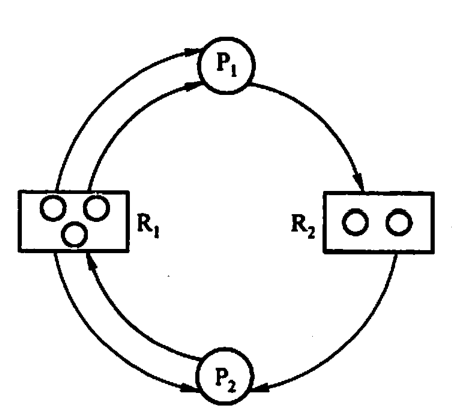
\includegraphics[width=0.3\textwidth]{./images/resource_allocation_graph.png}
  \caption{资源分配图示例}
  \label{resource_allocation_graph}
\end{figure}

资源分配图可以简化:
\begin{enumerate}
  \item 首先找出图中可以得到申请的资源的进程。如图\ref{resource_allocation_graph}的P$_1$申请了一个R$_2$资源,该资源空闲,P$_1$可以得到该资源。如果这种进程没有因得不到资源而阻塞,那么它迟早要运行结束,释放出已经得到的资源。于是将和这种进程相连的所有边删去。
  \item 由于资源的释放,与之相关的进程也可能解除了阻塞状态,考察这些进程,如果它们能够运行结束,就同样删去所有边。
  \item 如此循环,直到不能再删为止。如果此时没有边剩下,就说这个图是可以完全简化的。
  
  死锁等价于资源分配图不可完全简化。这叫做\textbf{死锁定理}。
\end{enumerate}

一些解除死锁的方法:
\begin{itemize}
  \item {\bf 资源剥夺法},挂起占有资源的\textbf{死锁}进程,将其资源剥夺,分配给其他进程。注意不能挂起太久。
  \begin{itemize}
    \item 不能剥夺非死锁的进程所所占有的资源。
  \end{itemize}
  \item {\bf 撤销进程法},直接杀掉占有资源的进程,将资源分给其他进程。杀的顺序可以是进程优先级或代价的高低。
  \item {\bf 进程回退法},OS保存进程的历史信息,要求一些进程主动回退,释放出一些资源。
\end{itemize}

\subsection{本章疑难点}

\textbf{饥饿进程}:和死锁不一样,指的是由于OS的分配策略不完美而引发某个进程一直等待的情况。例如在短进程优先调度中,短进程源源不断地进来,长进程一直排队而无法运行。如果饥饿进程被耽误的时间太长,导致即使完成也无济于事(有时效)时,称这个进程被“饿死”。

\section{内存管理}

\subsection{内存管理概念}

\subsubsection{内存管理的基本原理和要求}

内存管理的主要功能:
\begin{itemize}
  \item 内存空间的分配和回收
  \item 地址转换
  \item 内存空间扩充
  \item 内存共享:指多个进程访问内存的同一部分。
  \item 存储保护:保证各道作业在各自的存储空间内运行,互不干扰。
\end{itemize}

\begin{enumerate}
  \item {\bf 程序的链接和装入}
  
  程序的链接:
  \begin{itemize}
    \item 静态链接:编译时,链接所有模块
    \item 装入时动态链接:装入时,链接所有模块
    \item 运行时动态链接:运行时,根据需要链接模块。可加快程序的装入过程,同时节省大量的内存空间。
  \end{itemize}
  
  程序的装入:
  \begin{itemize}
    \item \textbf{绝对装入方式}:编译时直接确定装入的内存位置,装入后无需再修改程序和数据的地址。只能用于单道程序环境。
    \item \textbf{可重定位装入方式}:用于多道程序环境。装入时对逻辑地址修改得到物理地址,又称\textbf{静态(地址)重定位}。程序在内存中不能移动。
    \item \textbf{动态运行时的装入方式}:相对于上面的装入时进行重定位,本方式在程序执行时才进行重定位。又称\textbf{动态(地址)重定位}。需要重定位寄存器的支持。
  \end{itemize}

  \item {\bf 进程的内存映像}
  
  包括:
  \begin{itemize}
    \item 代码段:只读
    \item 数据段:包括全局变量和静态变量
    \item PCB
    \item 堆:从低地址向高地址生长。
    \item 栈:从高地址向低地址生长。
  \end{itemize}
  
  \begin{figure}
    \centering
    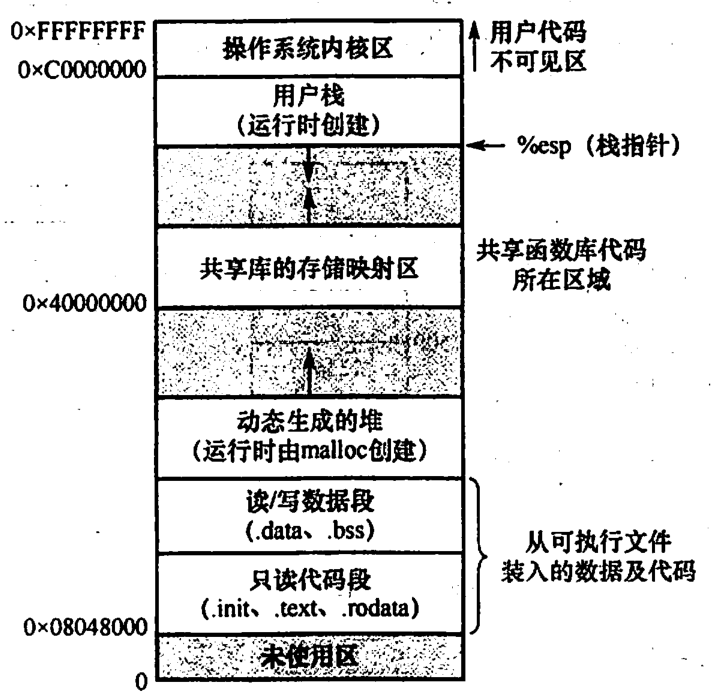
\includegraphics[width=0.5\textwidth]{./images/process_in_memory.png}
    \caption{内存中的一个进程}
  \end{figure}

  \item {\bf 内存保护}
  
  有两种方法:
  \begin{itemize}
    \item 在CPU中设置一对上下限寄存器,存放进程地址空间的上下界。
    \item 采用重定位寄存器(又称基地址寄存器)和界地址寄存器(又称限长寄存器)来实现。只有OS内核才能加载、修改这两个寄存器。
  \end{itemize}

  \item {\bf 内存共享}
  
  仅\textbf{只读}的区域才适合共享。

  \textbf{可重入代码}:又叫纯代码,指允许多个进程同时访问但不允许任何修改的代码。
\end{enumerate}

\subsubsection{覆盖与交换}

本节已从新大纲中删除。了解即可。参见24版王道书P177(书的P164)。

\textbf{覆盖技术}是早期在\textbf{单一连续存储管理}中使用的一种扩大存储容量的一种技术。也可用于\textbf{固定分区分配}方案。

\subsubsection{连续分配管理方式}

最早出现的一种存储器分配方式,该方式为用户分配一个连续的内存空间。

内存的零头:
\begin{itemize}
  \item 内零头:分配给进程,而进程未用到的内存部分;
  \item 外零头:未分配给进程,但因为太小而无进程能用;
\end{itemize}

\begin{enumerate}
  \item {\bf 单一连续分配}
  \begin{itemize}
    \item 基本思想:内存分为两个区域:一个供操作系统使用,一个供用户使用。在一段时间内,\textbf{只有一个进程在内存}。
    \item 三种典型的布局方式:
    \begin{itemize}
      \item 用户空间在低地址,系统空间在高地址。
      \item 和上面反过来。
      \item 系统空间在两边,把用户空间夹起来。
    \end{itemize}
    \item 实现:设置基址寄存器、限界寄存器,要求逻辑地址映射为物理地址后,物理地址必须在两者之间。
    \item 特点:简单,仅适用于单用户单任务OS。有内部碎片,存储器利用率极低。
  \end{itemize}
  \item {\bf 固定分区分配}
  \begin{itemize}
    \item 用于多道程序系统。把内存划分为固定的几个部分,维护一个分区使用表,按照分区大小进行排序。示例见表\ref{area_table_example}。
    \item 划分方法:
    \begin{itemize}
      \item 分区大小相等
      \item 分区大小不等,划分为多个较小的分区、适量的中等分区和较少的大分区。
    \end{itemize}
    \item 特点:
    \begin{itemize}
      \item 最早的支持多道程序的内存管理方式。
      \item 简单,现在仍在嵌入式系统中应用。
      \item 内零头严重。
    \end{itemize}
  \end{itemize}
  \item {\bf 动态分区分配}
  \begin{itemize}
    \item 基本思想:程序运行时划分大小合适的分区,程序结束后收回分区
    \item 配套数据结构:
    \begin{itemize}
      \item 空闲分区表:和固定分区一样
      \item 空闲分区链:在分区头部放入必要的说明信息和前向指针,分区尾部放入后向指针。
    \end{itemize}
    \item 动态分区分配算法:分为分配算法和回收算法两部分。分配算法又分基于顺序搜索的算法和基于索引搜索的算法两部分。
    \item 回收算法比较简单,在回收内存之后要做:
    \begin{itemize}
      \item 上下两个相邻区都是空闲区时,合并三个区
      \item 上空闲下不空闲时,合并上面的区
      \item 下空闲上不空闲时,合并下面的区
      \item 上下都不空闲时,不合并。
    \end{itemize}
    \item 基于顺序搜索的分配算法:用于小型系统
    \begin{itemize}
      \item 首次适应算法
      \begin{itemize}
        \item 低地址端被快速分配,碎片迅速出现
        \item 高地址端可能出现大块空闲区
      \end{itemize}
      \item 循环首次适应算法
      \begin{itemize}
        \item 下一次查找时,从上一次匹配的位置继续按照首次适应的方式查找。
        \item 需要设置一个查找指针
        \item 本质是CLOCK算法
        \item 碎片分布均匀
      \end{itemize}
      \item 最佳适应算法
      \begin{itemize}
        \item 找到一个够用且最小的分区。
        \item 需要将空闲区按照从小到大的顺序形成一个链,第一次找到的能放下的分区一定是最佳的。
        \item 碎片会迅速出现,实际上是很差劲的算法。
      \end{itemize}
      \item 最坏适应算法
      \begin{itemize}
        \item 仍然形成空闲分区链,但顺序是从大到小,每次只检查第一个(最大的)分区能否满足要求。
        \item 碎片出现最慢,但优先使用大内存块,导致很快就没有可用的大内存块了,同样是很差劲的算法。
      \end{itemize}
    \end{itemize}

    这里面最好的其实还是最简单的首次适应算法。

    \item 基于索引搜索的分配算法:用于大中型系统
    \begin{itemize}
      \item 快速适应算法
      \item 伙伴系统
      \item 哈希算法
    \end{itemize}
  \end{itemize}
  \item {\bf 可重定位分区分配}
  \begin{itemize}
    \item 在动态分区分配的基础上引入”紧凑“机制,消除外零头。使用动态地址重定位。
  \end{itemize}
\end{enumerate}

\begin{table}[!ht]
  \centering
  \caption{分区说明表示例}
  \label{area_table_example}
  \begin{tabular}{|c|c|c|c|}
  \hline
    \textbf{区号} & \textbf{分区长度(KB)} & \textbf{起始地址} & \textbf{状态} \\ \hline
    1 & 12 & 20 & 已分配 \\ \hline
    2 & 32 & 32 & 已分配 \\ \hline
    3 & 64 & 64 & 未分配 \\ \hline
    4 & 128 & 128 & 已分配 \\ \hline
  \end{tabular}
\end{table}

\subsubsection{基本分页存储管理}

与连续分配相对,有离散分配方式,分为以下三类:
\begin{itemize}
  \item 分页存储管理方式
  \item 分段存储管理方式
  \item 段页式存储管理方式
\end{itemize}

页面不宜太大,也不宜太小,太大内存利用率低,太小则会产生大量页面,导致页表很长,浪费内存。
一般为2的整数次方,1KB-8KB。

\begin{enumerate}
  \item {\bf 页表}
  
  每个进程都有一张。

  \begin{figure}[h]
    \centering
    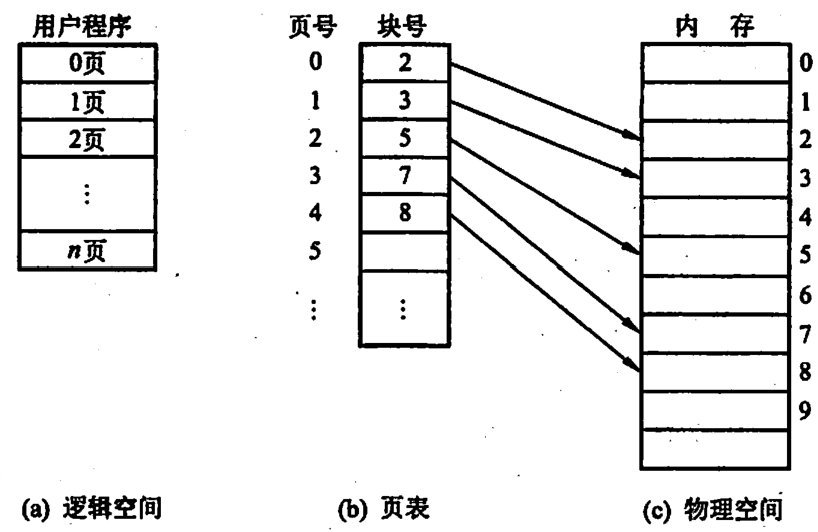
\includegraphics[width=0.6\textwidth]{./images/page-table.png}
    \caption{页表的作用}
  \end{figure}

  \item {\bf 基本地址变换机构}
  
  \begin{figure}[h]
    \centering
    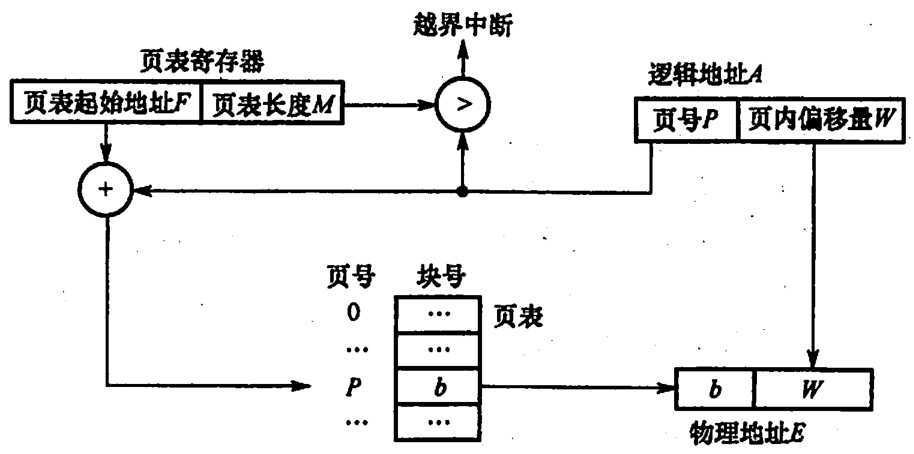
\includegraphics[width=0.6\textwidth]{./images/addr-translate.png}
    \caption{基本地址变换机构}
  \end{figure}

  系统中设置一个页表寄存器PTR,用于存储页表的起始地址F和页表长度M。这两个数据平时存在进程的PCB中,当进程运行时,调入PTR。

  地址变换是由硬件自动完成的。

  \item {\bf 带有TLB的地址变换机构}
  
  如果页表全部保存在内存中,那么取一次数据需要至少两次访存:访问页表一次,访问数据一次。

  在地址变换机构中引入一个有并行查找能力的Cache——快表TLB,其中保存一些页表项。相应地称内存中的页表为慢表。
  
  取数据时,先到TLB中查找,若命中则直接访存取数据,若不命中则查慢表,然后取数据并把这个页表项放进TLB。TLB满时,使用适当的算法进行淘汰。

  有些处理器设计成TLB和慢表同时检索,若TLB命中则停止查慢表。

  TLB的命中率一般可达90\%以上。

  \begin{figure}[h]
    \centering
    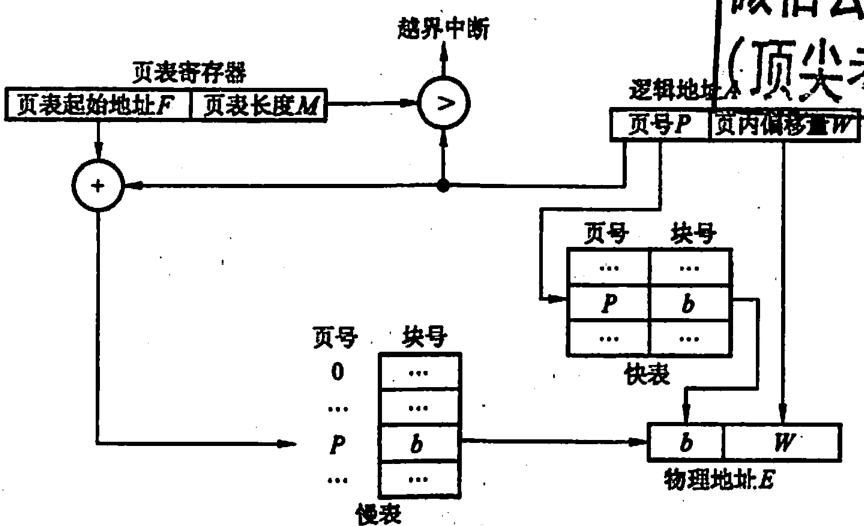
\includegraphics[width=0.6\textwidth]{./images/addr-translate-with-tlb.png}
    \caption{带有TLB的地址变换机构}
  \end{figure}

  \item {\bf 两级页表}
  
  单级页表在内存容量较大时,会占用很多空间。故引入多级页表。

  顶级页表\textbf{只能有一个页面}。
\end{enumerate}

\subsubsection{基本分段存储管理}

按照用户进程中的自然段划分逻辑空间。段内要求连续,段间不要求连续。逻辑地址=段号+段内偏移量

页式系统中内存管理对用户透明,段式系统中则要求编译器管理段号和偏移量。

\textbf{段表}:每个进程都有一张段表,其中的每个项对应进程的一段。包含3个域:段号、段长、本段在内存的起始地址。

这种方式是按照逻辑划分内存,有利于程序的动态链接。

\subsubsection{段页式管理}

段页式系统中,逻辑地址分为三部分:段号、页号和页内偏移量。

系统为每个进程建立一张段表,每个分段有一张页表。

地址变换时,先通过段表查找页表始址,然后通过页表查找到页帧号,最后形成物理地址,需要三次访存。

段页式管理的地址空间是\textbf{二维的}。

\begin{problem}
  ( \ \ )存储管理方式提供一维地址结构。
  \begin{enumerate}
    \item [A. ] 分段
    \item [B. ] 分页
    \item [C. ] 分段和分页
  \end{enumerate}
\end{problem}

\begin{solution}
  B. 确定一个地址需要几个参数,作业地址空间就是几维的。分页方式只需要给出页号。分段方式需要给出段号和段内地址。
\end{solution}

\begin{table}[h]
  \centering
  \begin{tabular}{|c|c|}
    \hline
    \textbf{管理方式} & \textbf{碎片情况} \\ \hline
    固定分区分配 & 内部碎片 \\ \hline
    分页 & 内部碎片 \\ \hline
    分段 & 外部碎片 \\ \hline
    段页式 & 内部碎片 \\
    \hline
  \end{tabular}
  \caption{不同内存管理方式产生的碎片情况}
\end{table}

\subsection{虚拟内存管理}

\subsubsection{虚拟内存的基本概念}

存储管理的两个基本问题:
\begin{itemize}
  \item 有的作业很大,不能完整装入内存。
  \item 作业很多,不能全部放入内存,但它们又要求同时运行。
\end{itemize}

程序运行的局部性原理:
\begin{itemize}
  \item {\bf 时间局部性}:刚执行过的指令在不久后很可能再次被执行,或程序刚访问过的数据很可能再次被访问。典型原因是程序中的循环。
  \item {\bf 空间局部性}:程序刚访问过某存储单元,则附近的存储单元也很可能被访问。典型原因是程序的顺序执行。
\end{itemize}

\textbf{定义}:虚拟存储器是指具有请求调入功能和置换功能,能从逻辑上对内存容量加以扩充的一种存储器系统。其逻辑容量由内存容量和外存容量之和决定,运行速度接近内存速度,而每位的成本由接近外存。

特征:
\begin{itemize}
  \item {\bf 多次性}。程序无须一次性全部装入内存,而是可以分多次装入。
  \item {\bf 对换性}。程序和数据无须常驻内存,在必要时可以换入换出。
  \item {\bf 虚拟性}。能从逻辑上扩展内存容量,使用户看到的容量远大于实际容量。
\end{itemize}

实现方法:
\begin{itemize}
  \item 请求分页系统
  \item 请求分段系统
  \item 请求段页系统
\end{itemize}

三种方法都需要一定的\textbf{硬件支持}:
\begin{itemize}
  \item 一定容量的内存和外存。
  \item 页表/段表机制,作为主要的数据结构。
  \item 中断机构。在缺页/段时产生中断。
  \item 地址变换机构,完成逻辑地址到物理地址的转换。
\end{itemize}

\subsubsection{请求分页管理方式}

\textcolor{blue}{“请求x式”是虚拟存储的同义词}。

为了应对页不在内存的情况,针对基本分页系统的页表结构进行扩充,形成如图\ref{page_request_system}的结构。

\begin{figure}[h]
  \centering
  \begin{tabular}{|c|c|c|c|c|c|}
    \hline
    页号 & 物理块号 & 状态位P & 访问字段A & 修改位M & 外存地址 \\
    \hline
  \end{tabular}
  \caption{请求分页系统中的页表项}
  \label{page_request_system}
\end{figure}

\begin{itemize}
  \item 状态位P:标示当前页面是否在主存。
  \item 访问字段A:记录一段时间内被访问的次数,供置换算法参考。
  \item 修改位M,标示该页面在被调入内存后是否被修改过。
  \item 外存地址:指出该页面在外存的地址。
\end{itemize}

请求分页系统的地址变换过程:图\ref{page_request_address_translation}

\begin{figure}
  \centering
  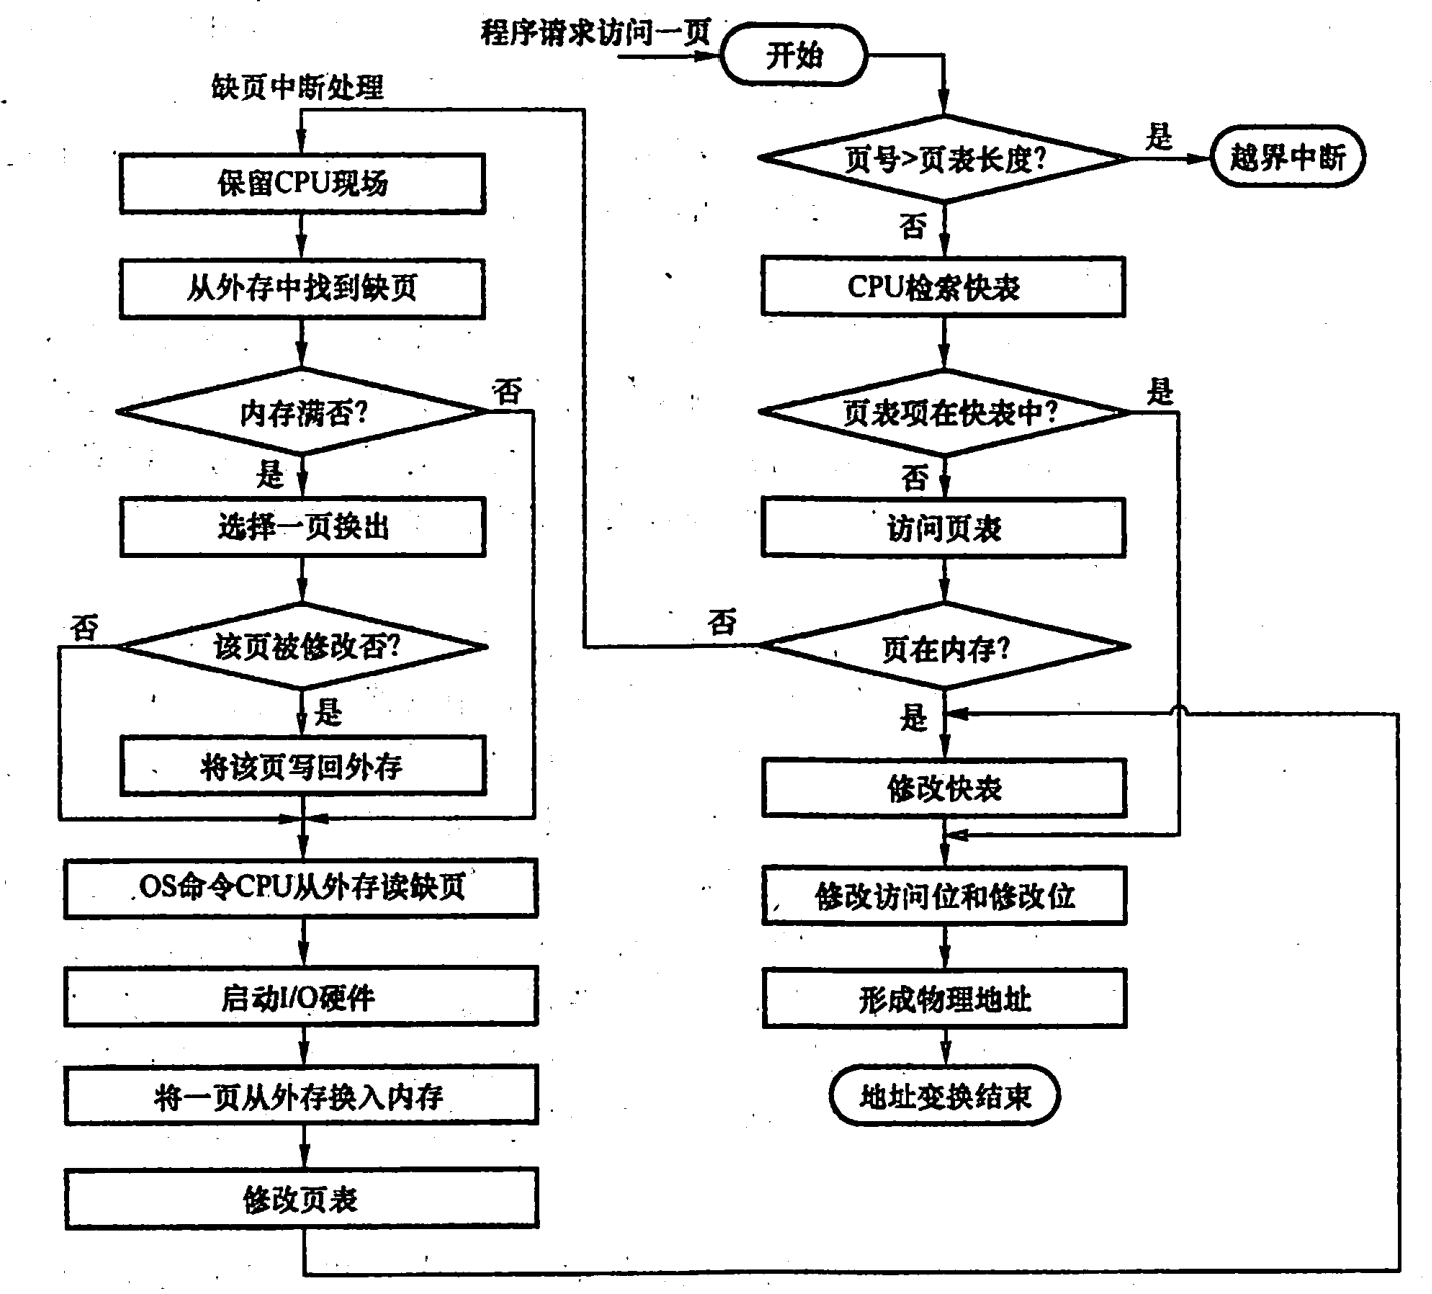
\includegraphics[width=0.7\textwidth]{./images/page_request_address_translation.png}
  \caption{请求分页系统中的地址变换过程}
  \label{page_request_address_translation}
\end{figure}

\subsubsection{页框分配}

\begin{enumerate}
  \item {\bf 驻留集}
  
  给一个进程分配的物理页框的集合,叫做这个进程的驻留集。

  \item {\bf 内存分配策略}
  
  \begin{itemize}
    \item 根据给进程分配的空间是否固定,可分为
    \begin{itemize}
      \item {\bf 固定分配}:给进程分配的物理块数目固定
      \item {\bf 可变分配}:给进程分配的物理块数目不固定
    \end{itemize}
    \item 根据缺页时的置换策略,可分为
    \begin{itemize}
      \item {\bf 全局置换}:系统从全局的空闲物理块中取出一块给进程,然后调页。
      \item {\bf 局部置换}:系统从该进程所属的空闲物理块中取出一块给进程,然后调页。
    \end{itemize}
  \end{itemize}
  
  将上面的两个维度组合,产生三种策略:
  
  \begin{itemize}
    \item {\bf 固定分配局部置换}
    \item {\bf 可变分配全局置换}
    \item {\bf 可变分配局部置换}
    \item 对进程进行固定分配时页面数不变,不可能出现全局置换。
  \end{itemize}

  \item {\bf 物理块调入算法}
  
  仅限于固定分配策略。
  \begin{itemize}
    \item 平均分配算法
    \item 按比例分配算法:按照进程的大小比例分配
    \item 优先级分配算法:按照进程的优先级分配,优先级高的分的多。
  \end{itemize}

  通常是将所有空闲物理块分成两部分:一部分按比例分,一部分按优先级分。
  
  \item {\bf 调入页面的时机}
  
  \begin{itemize}
    \item 预调页策略
    \item 请求调页策略
  \end{itemize}

  \item {\bf 从何处调入页面}
  
  请求分页系统的外存可分为两部分,一部分是连续分配的\textbf{对换区},一部分是离散分配的\textbf{文件区}。对换区一般比文件区快。发生缺页时:
  \begin{itemize}
    \item 若系统拥有足够的对换区空间,则全部从对换区调页。为此在运行前要把进程用到的文件都拷贝到对换区。
    \item 若系统缺乏足够的对换区空间,读比写快,因此只读的文件直接从文件区调入,用完需要淘汰页时直接扔了,不再换出;对于需要修改的页,从对换区调入。
    \item UNIX方式。
  \end{itemize}
\end{enumerate}

\subsubsection{页面置换算法}

选择换页时调出哪一页的算法称为页面置换算法。

\begin{enumerate}
  \item {\bf 最佳(OPT)置换算法}:理论上最优的算法
  \item {\bf 先进先出(FIFO)页面置换算法}:每次都淘汰在内存中驻留时间最久的页面。没有考虑局部性,因此效果不佳。还会出现分配的物理块数增多但页故障数不减反增的\textbf{Belady异常}现象。OPT和LRU则不会出现。该算法基于队列实现。
  \item {\bf 最近最久未使用(LRU)置换算法}:效果良好。该算法基于堆栈实现,需要额外的堆栈和寄存器硬件。可以证明,基于堆栈实现的算法不会出现Belady异常。
  \begin{itemize}
    \item LRU淘汰问题简便解法:对请求序列从后往前数【页框数】个\textbf{不同的}数,停止的数字就是要淘汰的页。
  \end{itemize}
  \item {\bf 时钟(CLOCK)置换算法}
  
  是低配的LRU,目的是用更少的硬件资源实现和LRU相近的性能。叫做CLOCK的原因是这种算法的工作方式就像钟表一样循环往复。
  \begin{itemize}
    \item {\bf 简单的CLOCK置换算法}
    
    为每页设置一个访问位A。将所有页视作一个循环队列,并设置一个替换指针。某一页被替换时,将指针指向该页的下一页。如果需要换页,则检查当前指向的页的访问位。如果是0,则换出;如果是1,则置为0(再给一次机会)。如此循环扫描,直到找到0为止。
    \item {\bf 改进的CLOCK置换算法}
    
    这种改进将页面是否被更改过也纳入了考虑。更改的页面需要真正写入磁盘,未更改的页可以简单丢弃,故更改的页换页代价更高。为每页再增加一个修改位M。扫描过程如下:
    \begin{enumerate}
      \item 第一趟扫描,寻找A=0且M=0的页。这种页替换代价最小,一旦找到就停止扫描,将该页换出。若未找到,则开始第二趟。这一趟\textbf{不修改A}。
      \item 第二趟扫描,寻找A=0且M=1的页。一旦找到就停止扫描,将该页换出。若未找到,则开始第三趟。这一趟\textbf{将所有=1的A置为0}。
      \item 第三趟扫描,将所有A置为0,然后按第一趟的逻辑扫描,若还不满足,则按第二趟的逻辑扫描。此时一定可以找到换出的页。
    \end{enumerate}
  \end{itemize}
\end{enumerate}

\subsubsection{抖动和工作集}

\textbf{抖动}:刚刚换入的页马上就要换出,刚刚换出的页马上就要换入,如此持续换页。

抖动发生的\textbf{根本原因是}:系统中的进程太多,分给每个进程的物理块太少。

\textbf{工作集}是指在某段时间内,进程要访问的页面集合。工作集的大小$W$可由工作集窗口$\Delta$和时间$t$确定。对于局部性好的程序,工作集的大小一般远远小于工作集窗口的大小。

\textcolor{blue}{所有的页面调度策略都不能完全避免抖动。}

为了避免发生抖动,一般要为进程分配大于其工作集的物理块数。

\section{文件管理}

\subsection{文件系统基础}

\subsubsection{文件的基本概念}

自底向上定义文件的结构:
\begin{itemize}
  \item {\bf 数据项},是最低级的数据组织形式。可分为:
  \begin{itemize}
    \item 基本数据项,是数据中的最小逻辑单位。
    \item 组合数据项,由多个基本数据项组成。
  \end{itemize}
  \item {\bf 记录},是一组相关的数据项的集合,用于描述一个对象在某方面的属性。
  \item {\bf 文件},是指由创建者所定义的、具有文件名的一组相关元素的集合。可分为:
  \begin{itemize}
    \item 有结构文件:由若干个相似的记录组成
    \item 无结构文件:是一个字符流,如二进制文件或字符文件。
  \end{itemize}
\end{itemize}

\subsubsection{文件控制块和索引结点}

\begin{enumerate}
  \item {\bf 文件的属性}
  
  OS通过文件控制块(FCB)来维护文件的属性。

  \begin{itemize}
    \item 文件名
    \item 文件类型
    \item 创建者
    \item 所有者
    \item 位置
    \item 大小
    \item 保护访问控制信息
    \item 创建时间、最后修改时间和最后存取时间。
  \end{itemize}

  \item {\bf 文件控制块 FCB}
  
  包含如下信息:
  \begin{itemize}
    \item {\bf 基本信息},如文件名、文件物理位置、文件的逻辑结构、文件的物理结构。
    \item {\bf 存取控制信息},如文件所有者的存取权限、核准用户的存取权限及一般用户的存取权限。
    \item {\bf 使用信息},如文件建立时间、上次修改时间等。
  \end{itemize}

  \item {\bf 索引结点}
  
  索引结点:查找文件目录时,要频繁访问硬盘,但查找文件实际上只需要文件名。因此可以将文件名单独抽取出来,搭配指向文件的指针,可以加速查找。这种文件名+指针的数据结构称为索引结点,也叫i节点(inode)。

  索引结点可以放在磁盘中,也可以预读入内存。
\end{enumerate}

\subsubsection{文件的操作}

\begin{enumerate}
  \item {\bf 文件的基本操作}
  
  下面的操作由OS通过系统调用提供。

  \begin{itemize}
    \item {\bf 创建}。有两个步骤:分配外存空间、为其创建目录项。
    \item {\bf 写文件}。通过系统调用完成。系统需要查找目录以找到文件,还要维护写指针。
    \item {\bf 读文件}。同上。维护读指针。一般一个进程不可能同时读和写同一个文件,因此读写指针可以合并起来。
    \item {\bf 重新定位文件}。查找指定的文件,并将读写指针复位。
    \item {\bf 删除文件}。找到文件对应的目录项,释放外存空间,并删除这一目录项。
    \item {\bf 截断文件}。也就是清空文件,但不删除文件。
  \end{itemize}

  \item {\bf 文件的打开与关闭}
  
  OS维护一个\textbf{打开文件表},其中保存有所有打开的文件的信息。
  
  用户可以通过\verb|open|系统调用向OS申请打开某个文件,OS根据文件名搜索目录,将文件的信息(包括该文件的物理位置)从外存复制到打开文件表的一个表目中,并将该表的索引返回给用户。
  
  用户再次使用该文件时,直接通过索引查到信息,免去再次搜索外存。
  
  用户不再使用文件时,通过\verb|close|系统调用关闭它,OS从打开文件表中删去对应的表目。

  在多个进程可同时打开文件的OS中,通常采用两级表:\textbf{整个系统表}和\textbf{每个进程表}。
  \begin{itemize}
    \item 整个系统表中保存所有FCB的副本和其他信息。
    \item 每个进程表中保存指向系统表相应条目的指针。
  \end{itemize}

  系统表中的表目采用引用计数方式管理。

  每个打开的文件都有如下关联信息:
  \begin{itemize}
    \item {\bf 文件指针},保存上一次访问文件时的访问位置(类似C语言中的文件指针),对每个打开文件的进程都是唯一的。
    \item {\bf 文件打开计数},即引用计数。
    \item {\bf 文件磁盘位置}
    \item {\bf 访问权限},同样对每个进程都是唯一的,保存在进程的表中。
  \end{itemize}
\end{enumerate}

\subsubsection{文件保护}

文件保护通过口令保护、加密保护和访问控制等方式实现。

\begin{enumerate}
  \item {\bf 访问类型}
  
  可加以控制的访问类型有:
  \begin{itemize}
    \item 读
    \item 写
    \item 执行
    \item 添加,将新信息添加到文件的末尾。
    \item 删除
    \item 列表清单,列出文件名和文件属性。
  \end{itemize}

  此外还有重命名、复制、编辑等。

  \item {\bf 访问控制}
  
  最常用的方法是根据\textbf{用户身份}进行控制。这当中最普通的方法是:为每个文件和目录增加一个\textbf{访问控制列表 ACL},规定\textbf{每个用户}的权限。
  \begin{itemize}
    \item 优点:可以管理复杂的访问方法
    \item 缺点:表长无法预计且可能导致复杂的空间管理
  \end{itemize}
  
  解决方法是使用\textbf{精简的访问列表}。它包含三种用户:
  \begin{itemize}
    \item {\bf 拥有者}:创建文件的用户
    \item {\bf 组}:一组拥有相同权限的用户
    \item {\bf 其他}:系统内所有其他用户
  \end{itemize}
  对这三种用户分别规定权限。

  其他的访问控制方式还有口令、密码等。

  现代OS中多使用多级目录结构,需要对目录也做访问控制。
\end{enumerate}

\begin{table}[h]
  \centering
  \caption{加密保护和访问控制机制的比较}
  \begin{tabular}{|c|c|c|}
    \hline
    & \textbf{加密保护} & \textbf{访问控制} \\ \hline
    \textbf{灵活性} & 相对低 & 相对高 \\ \hline
    \textbf{安全性} & 相对高 & 相对低 \\ \hline
    \textbf{实现} & 建议由用户程序实现 & 必须由OS实现 \\
    \hline
  \end{tabular}
\end{table}

\subsubsection{文件的逻辑结构}

\begin{itemize}
  \item 逻辑结构是从用户角度出发看到的文件组织形式。
  \item 物理结构(存储结构)是从实际角度出发看到的文件组织形式。
\end{itemize}

按照是否有结构,可将逻辑结构分为:
\begin{itemize}
  \item 有结构文件(记录式文件)
  \begin{itemize}
    \item 定长记录:检索容易
    \item 变长记录:灵活,但只能顺序查找。为此可以设置索引表,索引表本身是定长记录的。
  \end{itemize}
  \item 无结构文件(流式文件)
\end{itemize}

按照文件的组织方式,将\textbf{有结构文件}分为以下4类:
\begin{enumerate}
  \item {\bf 顺序文件}
  
  顺序文件的记录是定长记录或可变长记录。
  \begin{itemize}
    \item 最佳应用场合:对文件中的记录进行批量存取时。
    \item 若共有$N$个记录,则查找一个记录平均需要查$N/2$次。即查找性能不好。
    \item 此外添加或删除一个记录也很困难。可以引入一个事务文件,保存一段时间内的新增和删除记录,每隔一段时间进行实际写入。
  \end{itemize}

  为了访问顺序文件中的记录,必须首先找到记录的地址。有两种方法:
  \begin{itemize}
    \item 隐式寻址:就是从头找起,无论记录是定长的还是不定长的。
    \item 显式寻址:仅能用于寻址定长记录文件,直接将基址加上偏移量得到,由于定长,偏移量很容易得到。
  \end{itemize}
  \item {\bf 索引文件}
  \begin{itemize}
    \item 主要用于解决变长记录文件的快速查找问题。
    \item 方法:建立一张索引表,其中保存有每个记录的“指针”,是定长的,这样就可以按照关键字查找索引表,然后再跳转到实际记录。
    \item 也可以建立多个索引表,从而支持按照多个属性进行索引。
    \item 缺点是索引表须占用额外存储空间,尤其当记录数量很大时。
  \end{itemize}
  \item {\bf 索引顺序文件}
  \begin{itemize}
    \item 顺序文件和索引文件的一种折中。
    \item 将记录分组,为每组记录在索引表中建立一个项。
    \item 分组方式:按关键字分组,或直接按记录号分组。
    \item 查找过程:首先查索引表,找到待查项所在的组,通过指针跳转,再在组中顺序查找。
    \item 可以引入多级索引。
  \end{itemize}
  \item {\bf 直接文件或散列文件}
  \begin{itemize}
    \item 直接文件:直接给定记录的键值
    \item 散列文件:通过散列函数转换的键值决定记录的物理地址
    \item 没有顺序的特性
    \item 存取速度很快,但是可能会有冲突。
  \end{itemize}
\end{enumerate}

正规OS:顺序文件+暴露读写指针

\subsubsection{文件的物理结构}

文件的物理结构实际上就是研究文件数据在物理设备上是如何分布和组织的。这个问题有两个方面:
\begin{itemize}
  \item 文件的分配方式,讲的是\textbf{非空闲盘块}的管理。
  \item 文件的存储空间管理,讲的是\textbf{空闲盘块}的管理。
\end{itemize}

\begin{enumerate}
  \item {\bf 连续分配}
  
  每个文件是连续的。支持顺序访问和直接访问。
  \begin{itemize}
    \item {\bf 优点}:实现简单,存取速度快。
    \item {\bf 缺点}
    \begin{itemize}
      \item 文件长度难以动态增加
      \item 插入和删除记录时需要移动其他记录(类比顺序表)
      \item 反复增删文件后会出现外部碎片
      \item 文件需要的空间大小难以确定
    \end{itemize}
  \end{itemize}

  \item {\bf 链接分配}
  
  离散分配,消除了磁盘的外部碎片,提高了磁盘的利用率。又可分为隐式链接和显式链接两种。
  \begin{itemize}
    \item {\bf 隐式链接}
    
    目录项中含有文件第一个块和最后一个块的指针。除最后一块外,所有块都包含指向下一块的指针。这些指针对用户是透明的。

    只能顺序访问。

    改进:将几个盘块组成\textbf{簇(cluster)},代价是增加了内部碎片。用于大多数OS。
    \item {\bf 显式链接}
    
    指把链接指针拿出来放在一张表里。这个表在整个磁盘只设置一张,称为\textbf{文件分配表 FAT}。文件目录中存放文件的起始盘块号。

    \begin{figure}
      \centering
      \begin{tabular}{|c|c|}
        \hline
        \textbf{盘块号} & \textbf{下一块} \\ \hline
        0 & -2 \\ \hline
        1 & -1 \\ \hline
        2 & 8 \\ \hline
        3 & -2 \\ \hline
        4 & -2 \\ \hline
        5 & -1 \\ \hline
        6 & -2 \\ \hline
        7 & 1 \\ \hline
        8 & 5 \\ \hline
        9 & -2 \\ \hline
        $\cdots$ & $\cdots$ \\ \hline
      \end{tabular}
      \caption{FAT}
    \end{figure}

    可以用-1表示文件的最后一块,用-2表示空闲块。

    当进程请求分配磁盘块时,从FAT中找出-2的项分给进程。

    FAT在系统启动时读入内存,在内存中完成查找,速度快。
  \end{itemize}

  \item {\bf 索引分配} \label{index-allocation}
  
  将每个文件所有的盘块号集中在一起构成\textbf{索引块}。这个结构类似FAT表,但是每个进程都有一块。
  \begin{itemize}
    \item {\bf 优点}:支持直接访问,且没有外部碎片问题。
    \item {\bf 缺点}:由于索引块的分配,增加了系统存储空间的开销。
  \end{itemize}
  为了改善上述问题,可以使用如下方法:
  \begin{itemize}
    \item {\bf 链接方案}:索引块本身就是磁盘块。为了支持大文件,可以将多个索引块链接起来。
    \item {\bf 多层索引}
    \item {\bf 混合索引}
  \end{itemize}

  访问文件需要读两次外存,第一次读索引块,第二次读具体的块。为了加速,可以将索引块预读入内存。

  \item {\bf 混合索引分配}
  
  可以全面照顾到小、中、大、特大等多种文件。是UNIX采用的方式。
  \begin{itemize}
    \item {\bf 小型文件}。将小文件的所有盘块地址都放入FCB,进行直接寻址。
    \item {\bf 中型文件}。采用单级索引方式,即上面\ref{index-allocation}介绍的方式,将索引表存入FCB。
    \item {\bf 大、特大型文件}。采用两级或者三级索引方式。
  \end{itemize}
\end{enumerate}

\subsection{目录}

\subsubsection{目录的基本概念}

FCB的有序集合叫做文件目录。一个FCB就是一个文件目录项。

目录管理通过树形结构来解决和实现。

\subsubsection{目录结构}

\begin{enumerate}
  \item {\bf 单级目录结构}
  
  在整个文件系统中只建立一张目录表,每个文件占一个目录项。整个文件系统中不允许有重名的文件。不适用于多用户系统。查找速度慢、不便于共享。

  \item {\bf 两级目录结构}
  
  将目录按照用户分类,分为\textbf{主文件目录 MFD}(整个系统设置一个)和\textbf{用户文件目录 UFD}(每个用户一个)两级。MFD记录用户名和用户的UFD所在的位置,UFD记录具体的FCB。

  提高了检索速度,解决了多用户的文件重名问题,文件系统可以在目录上实现访问限制。但是也缺乏灵活性,不能对文件分类。

  \item {\bf 树形目录结构}
  
  这是从两级目录推广而来的。使用目录分隔符\verb|/|分隔目录,形成绝对路径或相对路径。

  可以方便地对文件进行分类,层次结构清晰,也能更有效地进行文件的管理和保护。

  这是目前大多数OS使用的方式。

  \item {\bf 无环图目录结构}
  
  树形目录便于实现文件分类,但不便于文件共享。
  
  对树形结构加以改造,让一些共享的结点独立出来,各个目录通过引用计数和写时复制来引用节点。使树形结构形成一个有向无环图。

  这种方式方便地实现了文件的共享,但使得系统的管理变得更加复杂。
\end{enumerate}

\subsubsection{目录的操作}

\begin{itemize}
  \item \textbf{搜索}。用户需要访问文件时,从目录中找到该文件。
  \item \textbf{创建文件}。即创建目录项,下同。
  \item \textbf{删除文件}。
  \item \textbf{创建目录}。在树形目录中还可以再创建目录。
  \item \textbf{删除目录}。有不删除非空目录和删除非空目录两种。
  \item \textbf{移动目录}。
  \item \textbf{显示目录}。即\verb|ls|。
  \item \textbf{修改目录}。即修改目录项的信息。
\end{itemize}

\subsubsection{目录实现}

本节带有星号,但王道书没有额外的说明。

常用的两种方法:
\begin{enumerate}
  \item {\bf 线性表}
  
  实现简单,查找比较费时。

  \item {\bf 哈希表}
  
  性能好,但需要避免冲突。
\end{enumerate}

目录查询需要大量磁盘I/O,为了提高性能,可以将当前目录复制到内存,以加速查找。

\subsubsection{文件共享}

常用的两种方法:硬链接和软链接。它们都属于静态共享。动态共享是有多个进程同时读写文件。
\begin{enumerate}
  \item {\bf 基于索引结点的共享(硬链接)}
  
  做一个索引结点,指向要共享的文件。每个引用文件的目录都在对应的目录项中放置指向索引节点的指针。此时目录项中不再保存元数据,而是保存在索引结点中。索引结点中还有引用计数。

  文件有一个所有者。所有者不再使用文件时,不能直接删除文件,而是将引用计数减一。如果直接删除文件,则其他引用文件的目录将会出现悬空指针。

  \item {\bf 基于符号链接的共享(软链接)}
  
  做一个\verb|LINK|类型的新文件,放到要共享的目录中。该文件只保存了真正文件的路径。如果要访问文件,则通过\verb|LINK|中的文件路径查找文件。这就是所谓的符号链接。

  文件所有者不再使用文件时,可以简单地删除。其他引用者发现\verb|LINK|中的路径不存在时,自动删除\verb|LINK|,也就不会产生悬空指针。
\end{enumerate}

\subsection{文件系统}

\textcolor{red}{本节包含大量2022考纲新增考点。}

\subsubsection{文件系统结构}

自底向上依次是:
\begin{enumerate}
  \item {\bf 设备}。
  \item {\bf I/O控制}。包括设备驱动程序和中断处理程序。驱动程序将输入的命令翻译成底层硬件的特定指令,硬件控制器利用这些指令和系统交互。驱动程序告诉控制器对设备的什么位置采取什么操作。
  \item {\bf 基本文件系统}。负责向对应的设备驱动程序发送通用命令,以读取和写入磁盘的物理块。
  \item {\bf 文件组织模块}。主要是将文件的逻辑地址转换为物理地址。
  \item {\bf 逻辑文件系统}。管理元数据,包括文件系统的结构、目录结构等。此外还负责文件保护。
  \item {\bf 应用程序}。
\end{enumerate}

见:图\ref{fs-layer}

\begin{figure}[h]
  \centering
  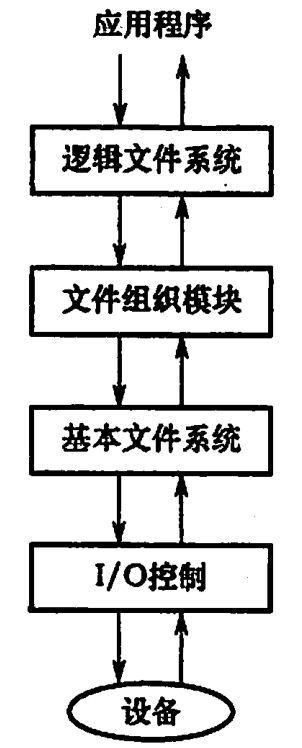
\includegraphics[width=0.15\textwidth]{./images/fs-layer.png}
  \caption{文件系统的层次结构}
  \label{fs-layer}
\end{figure}

\subsubsection{文件系统布局}

一块磁盘可能有多个分区,每个分区上都有一个独立的文件系统。

见:图\ref{fs-layout}

\begin{figure}[h]
  \centering
  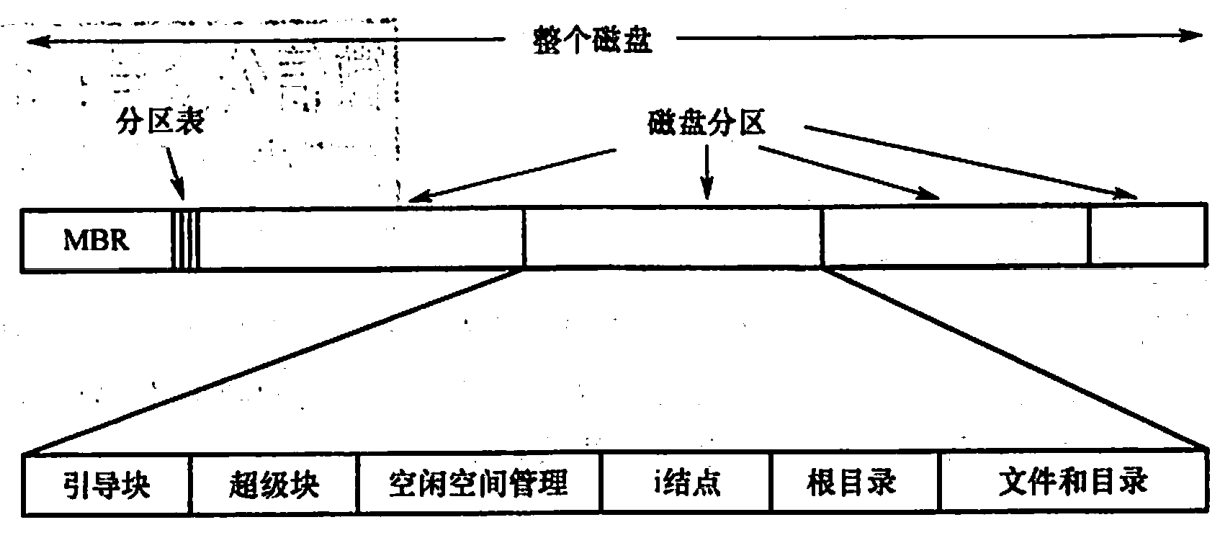
\includegraphics[width=0.7\textwidth]{./images/fs-layout.png}
  \caption{一个可能的文件系统布局}
  \label{fs-layout}
\end{figure}

\begin{itemize}
  \item {\bf 主引导记录 MBR}:位于0号扇区,用来引导计算机。MBR后面的分区表,给出每个分区的起始地址和结束地址。系统启动时,BIOS读入并执行MBR。MBR做的第一件事就是确定活动分区,读入引导块。
  \item {\bf 引导块}:是每个分区的第一个块。
  \item {\bf 超级块}:包含FS的所有关键信息,如块的数量和大小、空闲块的数量和指针、空闲FCB的数量和FCB指针等。计算机启动时或文件系统首次被使用时,超级块被读入内存。
\end{itemize}

\subsubsection{外存空闲空间管理}

包含文件系统的分区也叫\textbf{卷(volume)}。卷可以是磁盘的一部分,也可以是整个磁盘,也可以是多个磁盘组成的RAID。

在一个卷中,存放文件数据的空间和存放FCB的空间是分离的。

对文件存储设备的管理实质上是对空闲块的组织和管理。

\begin{enumerate}
  \item {\bf 空闲表法}
  
  这种方式和内存的动态分配很类似。属于连续分配方式,为每个文件分配连续的存储空间。系统建立一张空闲表,空闲区按照起始盘块号递增的次序排列。

  \begin{table}[!ht]
    \centering
    \caption{空闲表}
    \label{idle-table}
    \begin{tabular}{c|c|c}
    \hline
      \textbf{序号} & \textbf{第一个空闲盘块号} & \textbf{空闲盘块数} \\ \hline
      1 & 2 & 4 \\ \hline
      2 & 9 & 13 \\ \hline
      3 & 15 & 5 \\ \hline
      4 & \dots & \dots \\ \hline
    \end{tabular}
  \end{table}

  空闲区的分配方式有首次适应算法和最佳适应算法等。回收时也要考虑合并的问题。

  \item {\bf 空闲链表法}
  
  将所有空闲盘区拉成一条空闲链。根据基本元素是空闲块还是空闲区,可分为:
  \begin{itemize}
    \item {\bf 空闲盘块链}。用户需要盘块时,从链首分配相应数量的块给用户。用户返还时,将盘块放到盘块链的末尾。逻辑简单,但可能需要多次分配,而且链会很长。
    \item {\bf 空闲盘区链}。一般是用首次适应算法。优缺点恰好和上面相反。
  \end{itemize}

  \vspace*{10pt}

  上面提到的两种方法都不适合大型文件系统,因为表会太长。

  \item {\bf 位示图法}
  
  是一张$m\times n$的表,利用二进制的一位来表示一个盘块的使用情况。0表示空闲,1表示占用。位示图的行列可能从1开始编号,也可能从0开始,要特别注意。下面的例子是从1开始编号的。

  \begin{itemize}
    \item {\bf 盘块的分配}
    
    从头开始查找,直到找到需要的个数个空闲块。假设某空闲块是第$i$行第$j$列,则盘块号为
    \begin{equation*}
      b=n(i-1)+j
    \end{equation*}
    分配后勿忘将map[i,j]置为1。

    \item {\bf 盘块的回收}
    
    \begin{eqnarray*}
      i=(b-1)\ \text{DIV}\ n + 1 \\
      j=(b-1)\ \text{MOD}\ n + 1
    \end{eqnarray*}
    勿忘将map[i,j]置为0。
  \end{itemize}

  \item {\bf 成组链接法}
  
  UNIX使用的方法。结合了空闲表和空闲链表的特点,兼具二者优点,又克服了表太长的缺点。

  王道书原理没看懂

  \begin{figure}[h]
    \centering
    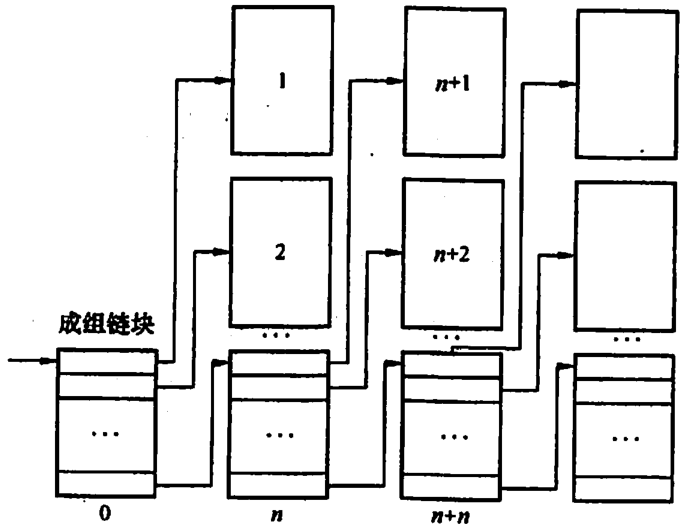
\includegraphics[width=0.5\textwidth]{./images/group-link-example.png}
    \caption{成组链接法示意图}
  \end{figure}

\end{enumerate}

\subsubsection{虚拟文件系统 VFS}

VFS为用户程序提供了FS操作的统一接口,屏蔽了不同FS的实现细节。VFS不是实际存在的FS,它只存在于内存中。VFS在系统启动时建立,在系统关闭时消亡。

用户程序可通过VFS的统一调用函数(如\verb|open|)等来操作不同的FS。

\begin{figure}[h]
  \centering
  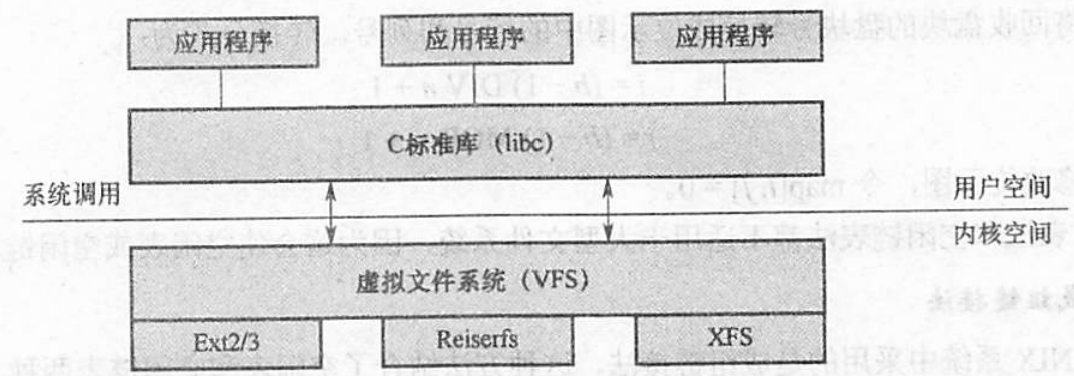
\includegraphics[width=0.7\textwidth]{./images/vfs.png}
  \caption{VFS示意图}
\end{figure}

VFS使用面向对象思想,抽象出一个通用的FS模型,定义了一些操作接口。新的FS只要实现这些接口,就可以纳入VFS工作。

\begin{figure}[h]
  \centering
  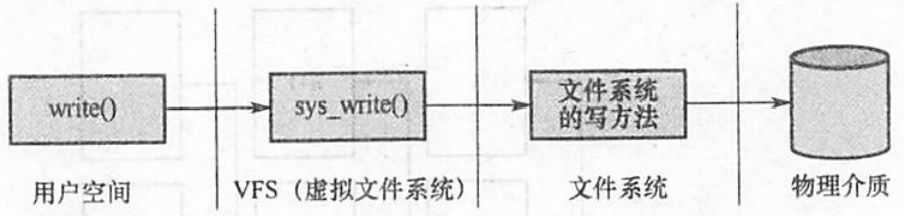
\includegraphics[width=0.6\textwidth]{./images/write-in-vfs.png}
  \caption{VFS中的write系统调用}
\end{figure}

VFS的另一个作用是提高系统性能。

\subsubsection{分区和安装}

\section{输入输出(I/O)管理}

本章考题比较简单,占比不大。

\subsection{I/O管理概述}

\subsubsection{I/O设备}

这一块内容比较混乱。

\begin{enumerate}
  \item {\bf 设备的分类}
  
  按照\textbf{信息交换的单位}分类,I/O设备可分为
  \begin{itemize}
    \item {\bf 块设备},以块为单位交换数据,属于有结构类型,如磁盘。可以随机寻址,速率较高。
    \item {\bf 字符设备},以字符为单位交换数据,属于无结构类型,如终端、打印机等。不可寻址,速率较低。多采用中断I/O。
  \end{itemize}
  
  按照\textbf{传输速率}分类,又可分为
  \begin{itemize}
    \item {\bf 低速设备},如键盘鼠标。
    \item {\bf 中速设备},如激光打印机。
    \item {\bf 高速设备},如磁盘机、光盘机。
  \end{itemize}

  \item {\bf I/O接口}
  
  I/O接口(设备控制器)位于CPU与设备之间。包括三部分:
  \begin{itemize}
    \item {\bf 设备控制器与CPU的接口},包括数据线、地址线和控制线。
    \item {\bf 设备控制器与设备的接口},一个设备控制器可以连接多个设备,因此有多个接口。每个接口都有数据、控制和状态三种类型的信号。
    \item {\bf I/O逻辑},通过一组控制线与CPU交互,用于实现对设备的控制。
  \end{itemize}

  \item {\bf I/O端口}
  
  是指设备控制器中可被CPU直接访问的寄存器。包括三类:
  \begin{itemize}
    \item {\bf 数据寄存器},实现CPU和外设之间的数据缓冲。
    \item {\bf 状态寄存器},获取执行结果和设备的状态信息。
    \item {\bf 控制寄存器},由CPU写入,以便启动命令或更改设备模式。
  \end{itemize}

  为了实现CPU与I/O端口的通信,可用两种方式:
  \begin{itemize}
    \item {\bf 独立编址},为每个端口分配一个I/O端口号,所有端口号形成一个端口空间。只有OS使用特定的I/O指令才能访问。
    \item {\bf 统一编址},为每个端口分配唯一的内存地址,通常靠近地址空间的顶端。可通过访问内存的方式访问端口。
  \end{itemize}

  \subsubsection{I/O控制方式}

  共4种
  \begin{figure}
    \centering
    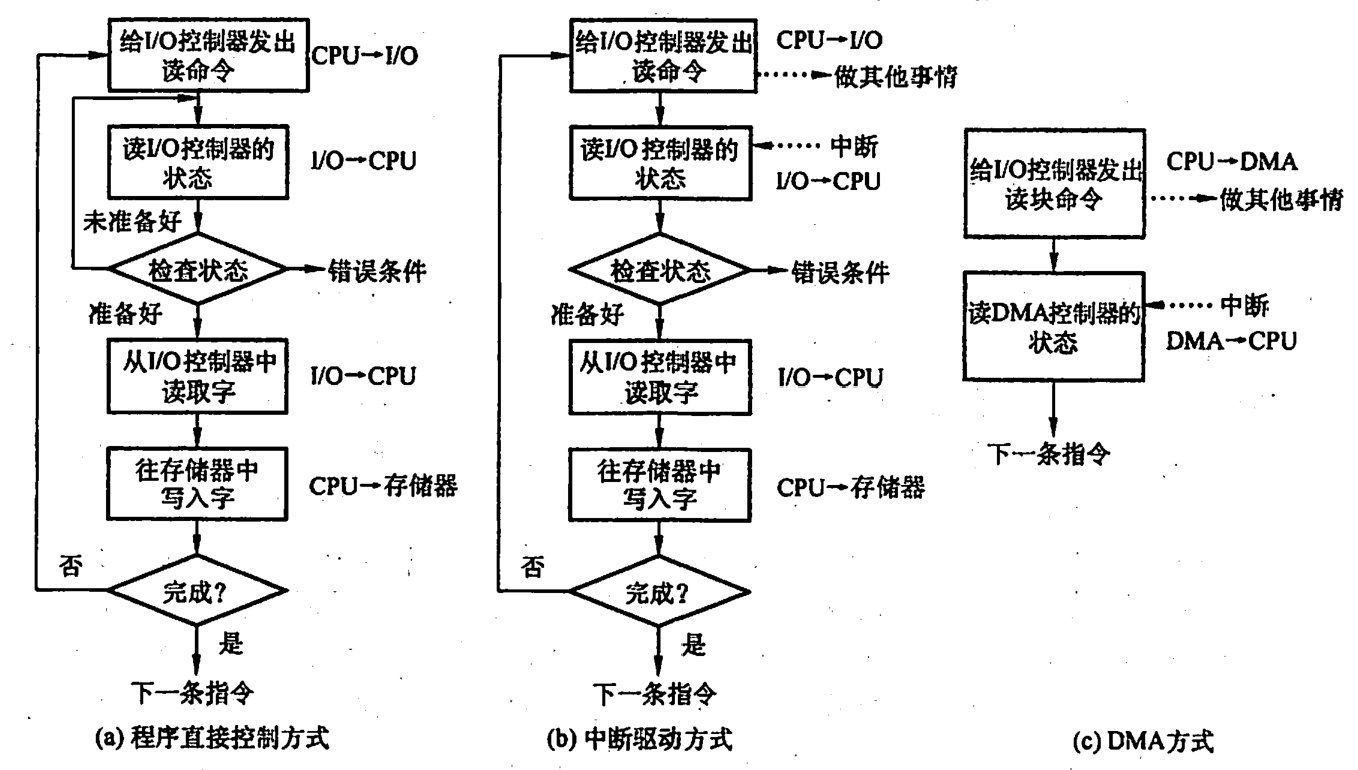
\includegraphics[width=0.7\textwidth]{./images/io-control.png}
    \caption{I/O控制方式}
  \end{figure}
  \begin{enumerate}
    \item {\bf 程序直接控制方式}
    
    就是轮询,逻辑简单,CPU和I/O设备串行工作,效率低下。

    \item {\bf 中断驱动方式}
    \item {\bf DMA方式}
    
    基本传输单位是数据块,数据块直接从设备传入内存(或者反之)。仅在传送一个或多个数据块的开始或结束时,才需要CPU干预。整块数据的传送是在DMA控制器的控制下完成的。
    \begin{figure}
      \centering
      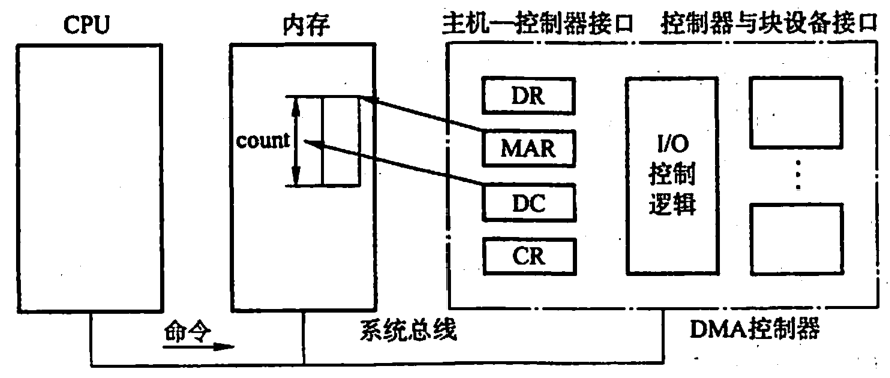
\includegraphics[width=0.7\textwidth]{./images/dma-controller.png}
      \caption{DMA控制器}
    \end{figure}

    \item {\bf 通道控制方式}
  \end{enumerate}
\end{enumerate}

\subsubsection{I/O软件结构}

\begin{figure}
  \centering
  \begin{tabular}{|c|}
    \hline
    用户层I/O软件 \\ \hline
    设备独立性软件 \\ \hline
    设备驱动程序 \\ \hline
    中断处理程序 \\ \hline
    硬件 \\ \hline
  \end{tabular}
  \caption{I/O层次结构}
  \label{io-layer}
\end{figure}

见:图\ref{io-layer}

设备独立性也叫设备无关性,是指应用程序独立于具体使用的物理设备的特性。为此引入逻辑设备与物理设备的概念。应用程序调用的是逻辑设备,然后将逻辑设备映射为物理设备。

使用逻辑设备名的好处是:
\begin{itemize}
  \item 增加设备分配的灵活性
  \item 容易实现I/O重定向
\end{itemize}

\subsubsection{应用程序I/O接口}

\begin{itemize}
  \item 字符设备接口,指的是数据的存取和传输是以字符为单位的设备,如键盘、打印机等。速率低,不可寻址,通常用中断方式。
  \item 块设备接口,典型设备是磁盘。速率较高、可寻址,通常用DMA方式。
  \item 网络设备接口
  \item 阻塞/非阻塞I/O。大部分OS提供的I/O接口都采用阻塞I/O。
\end{itemize}

\subsection{设备独立性软件}

\subsubsection{告诉缓存与缓冲区}

\begin{enumerate}
  \item {\bf 磁盘高速缓存}
  
  实际上是内存中的一块区域。可以是单独开辟的空间,也可以利用未分配的内存。

  \item {\bf 缓冲区}
  
  缓冲区可以用硬件实现,但由于成本原因,多采用内存缓冲区。

  若题目未明确说明,则通常认为缓冲区的大小和工作区的大小相等。
  
  假设从磁盘把一块数据输入到缓冲区的时间为$T$,操作系统将该缓冲区中的数据传送到用户区的时间为$M$,CPU对这一块数据的处理时间为$C$。

  根据系统设置缓冲器的个数,可分为以下4种(王道电子书P303):
  \begin{itemize}
    \item {\bf 单缓冲}
    
    分$T>C$和$T<C$两种情况讨论,可得出:单缓冲区处理每块数据的用时为$\max(C,T)+M$。

    \item {\bf 双缓冲}
    
    分$T<C+M$和$T>C+M$两种情况讨论,可得出:双缓冲区处理一块数据的用时为$\max(C+M, T)$。

    当两台机器之间只配置了单缓冲时,二者只能半双工通信。当两台机器之间配置了双缓冲时,二者可以全双工通信。

    \item {\bf 循环缓冲}
    
    若干个缓冲区构成一个循环队列。有两个指针in和out。
    \begin{itemize}
      \item 对于输入,in指向第一个空缓冲区,out指向第一个满缓冲区。
      \item 对于输出,正好相反。
    \end{itemize}
    
    \item {\bf 缓冲池}
  \end{itemize}
\end{enumerate}

\subsubsection{设备分配与回收}

\begin{enumerate}
  \item {\bf 设备分配概述}
  
  设备分配的总原则是让设备尽可能地忙碌,但又要避免由不合理的分配方式造成的死锁。
  \begin{itemize}
    \item {\bf 独占式使用设备}
    \item {\bf 分时式共享使用设备}
    \item {\bf 以SPOOLing方式使用外部设备}
  \end{itemize}

  \item {\bf 设备分配的数据结构}
  
  \begin{itemize}
    \item {\bf 设备控制表 DCT}
    \item {\bf 系统设备表 SDT}
    \item {\bf 控制器控制表 COCT}
    \item {\bf 通道控制表 CHCT}
  \end{itemize}

  \item {\bf 设备分配的策略}
  
  \begin{itemize}
    \item 设备分配原则。见上。
    \item 设备分配方式,可分:
    \begin{itemize}
      \item 静态分配方式,用户作业开始前,一次性分配该作业需要的全部设备资源,直至作业结束。不会有死锁,效率低下。
      \item 动态分配方式,根据需要进行分配,一旦用完立即释放,效率高,但设计不当可能造成死锁。
    \end{itemize}
    \item 设备分配算法,包括先请求先分配、优先级高者优先等。
  \end{itemize}

  独占设备多用静态分配方式,共享设备多用动态分配方式。

  \item {\bf 设备分配的安全性}
  \begin{itemize}
    \item {\bf 安全分配方式},进程发出I/O请求后立即阻塞,这样就无法发出新的I/O请求,设备分配安全,但CPU和设备是串行工作的。
    \item {\bf 不安全分配方式},进程发出I/O请求后继续运行,并可能发出新的请求。仅当进程请求的设备被占用时才阻塞。进程可以操作多个设备,运行高效,但可能造成死锁。
  \end{itemize}

  \item {\bf 逻辑设备名到物理设备名的映射}
  
  设置一张逻辑设备表LUT。其表项包括逻辑设备名、物理设备名和设备驱动程序入口地址。
  \begin{itemize}
    \item 整个系统只设置一张LUT,从而不允许系统中有重复的逻辑设备名,适合单用户系统。
    \item 每个用户设置一张LUT。
  \end{itemize}
\end{enumerate}

\subsubsection{SPOOLing技术(假脱机技术)}

SPOOLing技术引入的目的是缓和CPU的高速和I/O设备的低速之间的矛盾。

特点:
\begin{itemize}
  \item 提高了I/O的速度
  \item 将独占设备改造为共享设备
  \item 实现了虚拟设备功能
\end{itemize}

\subsection{磁盘和固态硬盘}

\subsubsection{磁盘}

扇区按照固定圆心角度划分,所以密度从最外道向里道增加,磁盘的存储能力受限于最内道的最大记录密度。

磁盘地址格式:柱面号·盘面号·扇区号

\subsubsection{磁盘的管理}

\begin{enumerate}
  \item {\bf 磁盘初始化}
  
  崭新的磁盘没有任何扇区划分。为崭新磁盘划分扇区的过程称为\textbf{低级格式化}。每个扇区通常由头部、数据区域和尾部组成。大多数磁盘出厂时就已经低级格式化过。低级格式化可以指定头部与尾部之间的数据区域的大小。

  \item {\bf 分区}
  
  OS在使用磁盘之前有两步操作:
  \begin{itemize}
    \item 将磁盘分为由一个或多个柱面组成的分区,分区的起始扇区和大小都记录在分区表中。
    \item 对物理分区进行逻辑格式化,即创建文件系统。
  \end{itemize}

  为了提高效率,OS常常将若干个扇区划分为一簇。一簇只能存放一个文件的内容。

  \item {\bf 引导块}
  
  系统启动时,从ROM中加载一个很小的装入程序,该程序到磁盘的固定位置查找引导程序,由引导程序完成复杂的启动工作。存放引导程序的块称为引导块。具有启动分区的磁盘称为启动磁盘或系统磁盘。

  \item {\bf 坏块}
  
  坏块不能恢复,只能屏蔽。
  \begin{itemize}
    \item 对于简单磁盘,采用手动屏蔽的方式。OS扫描磁盘,将坏块记录在FAT表中,程序不使用它们。
    \item 对于复杂磁盘,有控制器自行维护坏块表,该表在出场低格时已经初始化,并在使用过程中更新。低格还将保留一部分块作为备用,由控制器自动执行替换。
  \end{itemize}
\end{enumerate}

\subsubsection{磁盘调度算法}

一次磁盘读写的时间由三个因素决定。
\begin{itemize}
  \item {\bf 寻道时间$T_s$}。即磁头移动到指定磁道所需要的时间,也包括启动磁臂的时间。
  \begin{equation*}
    T_s=m\times n+s
  \end{equation*}
  其中,$m$是一个常数,约为0.2ms,$n$是跨越的磁道数量,$s$是磁臂启动时间,约为2ms。

  \item {\bf 旋转延迟时间$T_r$}。即磁头在目标磁道上等待,直到目标扇区到来为止的时间。设盘片旋转的速度为$r$,则(平均值)
  \begin{equation*}
    T_r=\frac{1}{2r}
  \end{equation*}
  对于典型的5400转硬盘,旋转一周的时间是11.1ms,则$T_r$是5.55ms。

  \item {\bf 传输时间$T_t$},即读出或写入数据消耗的时间。设要传输的字节数是$b$,盘片旋转速度为$r$,$N$是一个磁道上的字节数,则
  \begin{equation*}
    T_t=\frac{b}{rN}
  \end{equation*}
\end{itemize}

平均存取时间是上面三个值的和,但这个值没有太大意义,因为存取时间和调度算法密切相关。磁盘调度主要是在前两者即涉及“找”的部分做优化。传输时间是难以优化的。

常见的磁盘调度算法:
\begin{enumerate}
  \item {\bf 先来先服务算法 FCFS}
  
  谁先请求访问磁盘,谁就先访问。对于少量请求且访问聚簇的情况,有望达到较好性能,但在复杂请求条件下性能很差。

  \item {\bf 最短寻道时间优先算法 SSTF}
  
  总是选择离当前磁头最近的磁道。会有“饥饿”现象,即离磁头较远的磁道可能很久都不能访问。

  \item {\bf 扫描算法(电梯算法)SCAN}
  
  在当前磁头的\textbf{移动方向}上选择最近的磁道。访问局部性上不如前两者好,而且会偏向盘片最里和最外的请求。

  \item {\bf 循环扫描算法 C-SCAN}
  
  按照SCAN算法移动到磁盘边缘时,直接快速返回起始端,然后重新开始扫描,即只是单向处理。改进了SCAN算法偏向盘片最里和最外的请求的问题。

  \item {\bf LOOK和C-LOOK}
  
  这是SCAN和C-SCAN的改进算法。它们在访问到最靠边的请求时就返回,而不是傻傻地移动到磁盘边缘。

  如果题目没有特别说明,可以认为SCAN就是LOOK,C-SCAN就是C-LOOK。
\end{enumerate}

上面介绍的方法主要是减少寻道时间。为了减少延迟时间,可以对盘面扇区进行\textbf{交替编号},对磁盘片组中的不同盘面\textbf{错位命名}。解释见王道电子书P321。

\subsubsection{固态硬盘 SSD}

\begin{figure}
  \centering
  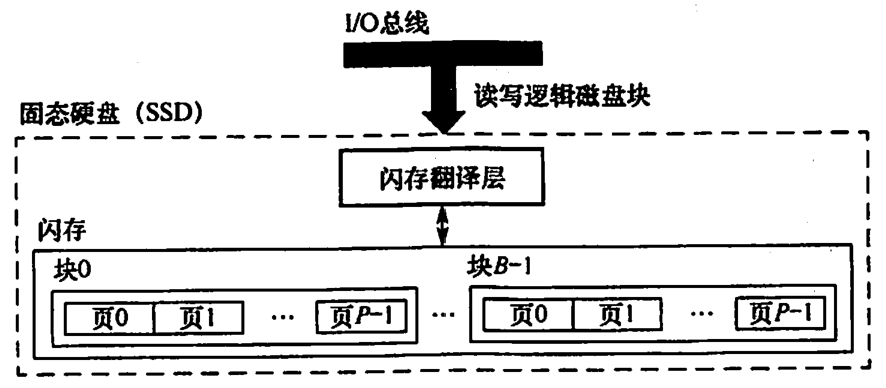
\includegraphics[width=0.7\textwidth]{./images/ssd.png}
  \caption{固态硬盘}
  \label{ssd}
\end{figure}

\begin{enumerate}
  \item {\bf SSD的特性}
  
  由一个闪存翻译层和若干个闪存芯片组成。在图\ref{ssd}中,一个闪存由$B$块组成,每块由$P$页组成。通常,一页的大小是512B~4KB,每块由32-128页组成,块的大小为16KB~512KB。数据是以页为单位读写的,但是以块为单位擦除的。一旦某个块被擦除,那么块中的页就可以再写入。某块擦除若干次(典型值为几百到数千次)后就会损坏。

  SSD的随机写比较慢,因为:
  \begin{itemize}
    \item 擦除块比较慢,往往比读取慢一个数量级。
    \item 写入某页时,必须将这个块中所有的页都复制到一个新块中,然后整体擦除。
  \end{itemize}

  \item {\bf 磨损均衡(Wear Leveling)}
  
  如果读写数据时只集中到闪存的某一部分,那么这部分会迅速磨损。当闪存的一小部分损坏后,整个闪存可能也会随之损坏。于是引入了磨损均衡技术:
  \begin{itemize}
    \item 动态磨损均衡。写入数据时,优先选择磨损程度较低的块。
    \item 静态磨损均衡。在没有写入任务时,由主控自动地将冷数据存入老块,让新块承担更多的写入。
  \end{itemize}
\end{enumerate}

\vspace*{30pt}

\begin{center}
  \Large{THE END}
\end{center}

\end{document}